% Copyright (c) 2017 Ongun Kanat <ongun.kanat@gmail.com>
% Permission is hereby granted, free of charge, to any person obtaining a copy of 
% this software and associated documentation files (the "Software"), to deal in 
% the Software without restriction, including without limitation the rights to 
% use, copy, modify, merge, publish, distribute, sublicense, and/or sell copies of 
% the Software, and to permit persons to whom the Software is furnished to do so, 
% subject to the following conditions:
% 
% The above copyright notice and this permission notice shall be included in all 
% copies or substantial portions of the Software.
% 
% THE SOFTWARE IS PROVIDED "AS IS", WITHOUT WARRANTY OF ANY KIND, EXPRESS OR 
% IMPLIED, INCLUDING BUT NOT LIMITED TO THE WARRANTIES OF MERCHANTABILITY, FITNESS 
% FOR A PARTICULAR PURPOSE AND NONINFRINGEMENT. IN NO EVENT SHALL THE AUTHORS OR 
% COPYRIGHT HOLDERS BE LIABLE FOR ANY CLAIM, DAMAGES OR OTHER LIABILITY, WHETHER 
% IN AN ACTION OF CONTRACT, TORT OR OTHERWISE, ARISING FROM, OUT OF OR IN 
% CONNECTION WITH THE SOFTWARE OR THE USE OR OTHER DEALINGS IN THE SOFTWARE.

% 12pt and ISO A4 paper with title page add notitlepage for otherwise
\documentclass[a4paper, 12pt, titlepage]{article}

% Margins and page size
\usepackage[a4paper,top=2.5cm,bottom=2.5cm,left=3.3cm,right=2.2cm]{geometry}

% Page headers are set to top right
\usepackage{fancyhdr}
\pagestyle{fancy}
\setlength{\headheight}{15pt}
\renewcommand{\footrulewidth}{0pt} % clear rulers
\renewcommand{\headrulewidth}{0pt}
\lhead{} % Empty left header
\rhead{\thepage} % Page number at the right header
\cfoot{} % Clear center of the footer

% Use American English for dates etc.
%\usepackage[american]{babel}
% If document is in Turkish then use
% \usepackage[turkish]{babel}
% or for both
\usepackage[turkish,american]{babel}

% Indent at section beginnings
%\usepackage{indentfirst}

% utf-8 support
\usepackage[utf8]{inputenc}


% Figure placement
\usepackage{float}

% An enumeration package for flexible enumeration
\usepackage{enumitem}

% Helvetica Sans-serif fonts
\usepackage{helvet}
\usepackage{sectsty}
\allsectionsfont{\normalfont\sffamily\bfseries}
\sectionfont{\fontsize{18pt}{21.6pt}\sffamily\bfseries}
\subsectionfont{\fontsize{16pt}{19.2pt}\sffamily\bfseries}
\subsubsectionfont{\fontsize{14pt}{16.8pt}\sffamily\bfseries}

% Paragraph spacings
\setlength{\parindent}{0pt}
\setlength{\parskip}{12pt}

% Courier monospace font
\usepackage{courier}

% Table of contents dot fill
\usepackage{tocloft}
\renewcommand{\cftsecleader}{\cftdotfill{\cftdotsep}}
\tocloftpagestyle{fancy}
\renewcommand{\cfttoctitlefont}{\sffamily\Large\bfseries}
\setlength{\cftbeforesecskip}{6pt}

% Links, both local and external
\usepackage{hyperref}
\hypersetup{
    unicode=true,
    colorlinks=true,
    urlcolor=blue,
    citecolor=black,
    menucolor=black,
    linkcolor=black
}

% Figure captions are bold
\usepackage[labelfont=bf,font=sf]{caption}


% Pseudocode from algorithmicx package
\usepackage{algorithmicx}
\usepackage{algpseudocode}
\usepackage[section,boxed]{algorithm}
\captionsetup[algorithm]{labelfont=bf,font=sf,justification=centering,position=top}

% For fitting tables into the page width
\usepackage{makecell}
\renewcommand{\theadalign}{cc} % Centering and at the middle
\renewcommand{\theadfont}{\bfseries} % Bold table headers
\usepackage{tabularx}
\newcolumntype{Y}{>{\centering\arraybackslash}X}

% Listings for implemented code
\usepackage{listings}
\lstset{basicstyle=\ttfamily,frame=lines,tabsize=4}
\renewcommand{\lstlistingname}{Listing}
\lstset{
    breakatwhitespace=false,
    breaklines=true,
    captionpos=b,
    escapeinside={\%*}{*)},
    frame=single,
    keepspaces=true,
    numbers=left,
    numbersep=5pt,
    xleftmargin=8pt,
}

% A powerful math notation package
\usepackage{amsmath}

% Override here with the names
\newcommand{\thetitle}{TinyNPU}
\newcommand{\theturkishtitle}{TinyNPU}
\newcommand{\theauthor}{Fırat Kızılboğa}
\newcommand{\thestudentid}{150200115}
\newcommand{\thedate}{March 2026}
\newcommand{\theturkishdate}{Mart 2026}
\newcommand{\theadvisor}{Assoc. Prof. Dr. Ayse Yilmazer}

\usepackage{color}
\definecolor{darkgreen}{RGB}{0, 128, ,0}
\newcommand{\fixme}[1]{{\color{red}\bfseries\sffamily (FIXME: #1)}}
\newcommand{\suggest}[1]{{\color{darkgreen}\bfseries\sffamily (SUGGESTION: #1)}}
\newcommand{\ask}[1]{{\color{blue}\bfseries\sffamily (QUESTION: #1)}}

\newcommand\Includegraphics{\expandafter\includegraphics\expandafter} 

% Title, author and date info
\title{\thetitle}
\author{\theauthor}
\date{\thedate}

% Graphics for PDFTeX
\usepackage{graphicx}


\begin{document}
\numberwithin{figure}{section}
\numberwithin{table}{section}
\numberwithin{lstlisting}{section}
\shorthandoff{=}


\begin{titlepage}
    \bfseries % Make all text bold in this environment
    \sffamily % Similarly select sans-serif font
    \begin{center}
        \LARGE{\textbf{ISTANBUL TECHNICAL UNIVERSITY \\ 
               FACULTY OF COMPUTER AND INFORMATICS} } \\
        \vspace{5.5cm}
        \LARGE{\thetitle}  \\
        \vspace{4.5cm}
        \Large{Graduation Project Final Report} \\
        \vspace{0.5cm}
        \Large{\theauthor} \\
        \Large{\thestudentid} \\
        \vspace{4cm}
        \large{Department: Computer Engineering} \\
        \large{Division: Computer Engineering} \\
        \vspace{1.5cm}
        \large{Advisor: \theadvisor} \\
        \vspace{\fill} % Fill out until the page end
        \large{\normalfont \sffamily \thedate}
    \end{center}
\end{titlepage}

\pagenumbering{Roman} % Capital roman numerals as page numbers
\newpage
\section*{Statement of Authenticity}
I/we hereby declare that in this study
\begin{enumerate}
    \item all the content influenced from external references are cited clearly and in detail,
    \item and all the remaining sections, especially the theoretical studies and implemented software/hardware that constitute the fundamental essence of this study is originated by my/our individual authenticity.
\end{enumerate}
\vspace{1em}
İstanbul, \theturkishdate
\vspace{3em}\\ \theauthor

\newpage
\section*{Acknowledgments}
I would like to thank my advisor, Assoc. Prof. Dr. Ayse Yilmazer, for her guidance throughout this project. I also thank the people whose open-source tooling and research made it possible to build, analyze, and validate the TinyNPU hardware and software stack.

\newpage
\section*{\centering\thetitle}
\centerline{\fontsize{16pt}{21.6pt}\sffamily\bfseries (SUMMARY)}
TinyNPU is a compact neural-network accelerator built and evaluated as a full hardware/software system. It combines an output-stationary systolic-array accelerator with a segmented compiler and runtime, a quantized model-preparation flow, and RTL-backed validation.

The hardware centers on an $N \times N$ systolic array, a unified buffer, an instruction memory, streamer logic, and a post-processing unit that performs bias addition, rescaling, activation, and packed writeback. The software traces PyTorch models, partitions them into accelerator segments and explicit scalar operations owned by the core, lowers supported segments into TinyNPU instruction and buffer images, and executes the result on the attached CV32E40P core.

This report treats the whole stack as the useful unit of design. Tensor layout, quantization boundaries, scalar core operations, runtime overhead, and realizable clock frequency all affect whether the accelerator is practical to use. The implemented system is validated on trained MNIST-derived MLP and convolution models, controlled multi-tile GEMM benchmarks, small transformer-like blocks, and synthesis/timing experiments that expose the system limits.

\newpage
\section*{\centering\theturkishtitle}
\centerline{\fontsize{16pt}{21.6pt}\sffamily\bfseries (ÖZET)}
TinyNPU, sistolik dizi tabanlı bir nöral işlemci birimini onu kullanılabilir hale getiren derleyici, çalışma zamanı, niceleme akışı ve benzetim tabanlı doğrulama ortamıyla birlikte ele alan bütünleşik bir donanım-yazılım sistemidir. Amaç yalnızca küçük bir hızlandırıcı çekirdeği tasarlamak değil, bu çekirdeği gerçek bir makine öğrenmesi iş akışında kullanılabilir hale getirmektir. Bu nedenle sistem, PyTorch tabanlı model hazırlama sürecini destekleyen, nicelemeli modelleri hızlandırıcı segmentlerine dönüştüren, desteklenmeyen işlemleri ana işlemci üzerinde çalıştıran ve sonuçları yazılım referanslarıyla doğrulayan bir yapı olarak tasarlanmıştır.

Donanım tarafında TinyNPU, birleşik tampon bellek ve komut belleği ile beslenen sistolik dizi tabanlı bir hesaplama çekirdeği etrafında kurulmuştur. Girdi aktivasyonları ve ağırlıklar birleşik tampondan akıtıcı birimlere, oradan da sistolik diziye iletilir. Hesaplama sonucunda oluşan değerler son işleme biriminden geçirilerek paketlenmiş biçimde tekrar belleğe yazılır. Bu yapı, yoğun nicelemeli matris işlemleri için verimli bir veri yolu sağlarken, dışarıdan görülen programlama modelini de yönetilebilir düzeyde tutmaktadır. Yazılım tarafı ise yüksek seviyeli model işlemlerini hızlandırıcı segmentleri ve gerekirse ana işlemci işlemlerini birlikte içeren bir yürütme planına dönüştürmektedir.

Bu çalışmada sistem, eğitilmiş MNIST tabanlı MLP ve evrişim modelleri, kontrollü GEMM deneyleri, küçük transformer benzeri bloklar ve sentez/zamanlama deneyleri üzerinde doğrulanmıştır. Ayrıca, hızlandırıcının gerçek hesaplama çevrimlerini paketleme, arayüz, çalışma zamanı ve saat frekansı maliyetlerinden ayıran bir ölçüm altyapısı kurulmuştur. Böylece çekirdeğin kendi verimliliği ile entegrasyon maliyetleri ayrı ayrı değerlendirilebilmektedir. Tekrarlı çıkarım senaryoları için oturum tabanlı çalışma ve ağırlık kalıcılığı desteği de eklenmiştir.

Rapor, bu sistemi donanım mimarisi, model hazırlama ve derleme akışı, doğrulama yöntemi ve deneysel sonuçlarıyla birlikte sunmaktadır. Sonuçlar, sistolik çekirdeğin güçlü hesaplama sağladığını, ancak toplam davranışın hâlâ veri yerleşimi, bölütleme ve çalışma zamanı maliyetlerine duyarlı olduğunu göstermektedir.

\newpage
\tableofcontents
\newpage

% For the ones who doesn't know: 1,2,..9 called West Arabic numbers
\pagenumbering{arabic}
\section{Introduction and Project Summary}
\subsection{Background and Motivation}
Modern deep neural networks demand substantial compute and memory bandwidth even at inference time. This has made specialized accelerator design a central topic both for datacenter-scale systems and for smaller edge-oriented deployments \cite{jouppi2017datacenter, genc2021gemmini}. Quantization is one of the main techniques that makes such deployment practical, because it reduces memory traffic and allows arithmetic throughput to increase when narrow integer types are used instead of floating-point data.

However, quantization is not a single fixed target. Mixed-precision work has shown that different layers or kernels inside the same model can tolerate different bit-widths \cite{wu2018mixedprecision}. This creates a hardware opportunity and a software problem at the same time. Hardware should benefit from narrower arithmetic when it is safe to do so, but the software stack must still prepare the model, preserve numerical intent, and decide where accelerator execution ends and scalar execution on the core begins.

\subsection{Problem Definition}
The main problem addressed by TinyNPU is not only how to build a small systolic-array accelerator, but how to make mixed-precision quantized computation usable from a real model flow. Fixed-precision accelerators leave throughput on the table when different parts of a model tolerate different bit-widths. Processor-centric low-bit approaches, on the other hand, still pay software-side cost for packing, unpacking, and data movement around the arithmetic \cite{garofalo2021xpulpnn, armeniakos2024mixedprecision, reggiani2023mixgemm, fornt2025mixgemm}.

This project therefore treats the problem as a co-design task. The hardware must expose a regular packed-integer datapath, and the compiler/runtime must make tensor layout, quantization boundaries, and scalar core work explicit. The result should be measurable honestly, with accelerator compute, runtime overhead, and scalar core work kept separate.

\subsection{Project Scope and Approach}
TinyNPU approaches this problem with four coupled components:
\begin{enumerate}
    \item \textbf{A parameterized mixed-precision accelerator:} TinyNPU is centered around an output-stationary $N \times N$ systolic array, a unified buffer, streamer logic that feeds the array, and a post-processing unit that performs bias addition, rescaling, activation, saturation, and packed writeback.
    \item \textbf{Packed integer computation:} The processing elements support packed INT16, INT8, and INT4 execution modes. Throughput therefore scales with precision reduction, not by changing the global architecture, but by packing more useful work into the same datapath.
    \item \textbf{A segmented compiler/runtime:} The software flow traces supported PyTorch models, partitions them into accelerator segments and explicit scalar operations owned by the core, lowers legal accelerator work into instruction and buffer images, and executes the resulting plan on either software emulation or RTL simulation.
    \item \textbf{Verification and measurement infrastructure:} The project includes compiler-owned expected tensors, runtime verification points, repeated-run sessions, and benchmark accounting that separates accelerator compute from protocol and software overhead.
\end{enumerate}

TinyNPU runs trained MNIST-derived MLP and convolution models through the full compiler/runtime stack, benchmarks controlled multi-tile GEMM workloads, and evaluates small GPT/Llama-like blocks to study transformer lowering. These experiments expose both the arithmetic capability of the accelerator and the system-level cost of staging, boundaries, scalar core operations, timing closure, and runtime service.
\newpage

\section{Comparative Literature Survey}
\subsection{Mixed-Precision Quantization}
Mixed-precision quantization work is the clearest algorithmic motivation for TinyNPU. Wu et al. formulate layer-wise quantization as a search problem and show that different layers can be assigned different bit-widths without treating the whole model uniformly \cite{wu2018mixedprecision}. This is the key observation behind a variable-precision accelerator: if model layers do not all need the same precision, a fixed-precision datapath cannot exploit the full efficiency opportunity.

Quantization is also relevant as a compiler concern rather than only a hardware concern. SmoothQuant is an example of pushing difficult numerical adjustments into an offline transformation so that runtime execution becomes simpler and more hardware-friendly \cite{xiao2023smoothquant}. TinyNPU follows the same general philosophy even though it does not implement the full SmoothQuant method itself: model preparation, fused rescaling, and compiler-ready conversion are treated as software responsibilities that simplify the accelerator contract.

\subsection{High-Performance Matrix Multiplication}
The mathematical core of TinyNPU is still matrix-style computation, so the project is strongly informed by classical GEMM literature. Goto and van de Geijn show that high-performance matrix multiplication depends not only on arithmetic throughput, but on careful tiling and data movement through the memory hierarchy \cite{goto2008anatomy}. The same principle appears in TinyNPU at a smaller scale. When matrices exceed the dimensions of the systolic array, the compiler and runtime must tile along the $M$, $N$, and $K$ dimensions while preserving the data reuse pattern expected by the array and its post-processing path.

\subsection{Existing Accelerator Architectures}
On the accelerator side, Google's TPU remains the canonical reference for systolic-array-style matrix acceleration \cite{jouppi2017datacenter}. Gemmini is especially relevant because it demonstrates how a systolic array, programming model, and system context can be treated as one full-stack research object rather than as an isolated RTL block \cite{genc2021gemmini}. That full-stack perspective is one of the strongest methodological reference points for TinyNPU.

An educational TinyTPU implementation was a useful starting point for understanding systolic-array organization, but it was not enough for this project \cite{chin2025tinytpu}. Extending the design toward mixed precision, tiled execution, and explicit post-processing exposed the need for a custom software contract, explicit core/accelerator boundaries, and a compiler/runtime that owns packing and verification.

Taken together, these references define TinyNPU's design space. It is not trying to outscale industrial accelerators. Its goal is a compact mixed-precision accelerator system whose hardware, compiler/runtime, and measurement boundary can be studied together on one working platform.
\newpage

\section{Developed Approach and System Model}
The system is described here as one CV32E40P-plus-accelerator platform with four cooperating subsystems: TinyNPU hardware, model preparation, compilation, and firmware execution. CV32E40P is the OpenHW CORE-V continuation of the RI5CY/PULP-class 32-bit RISC-V core lineage \cite{gautschi2017ri5cy}. In the reported implementation, the useful local system is the firmware core plus the matrix accelerator, not the matrix RTL block alone. A larger deployment could attach this subsystem to an external host through an SoC interconnect, AXI-style fabric, PCIe bridge, or another platform-specific interface. That outer system interface is intentionally left abstract; the measurements in this report are taken at the implemented TinyNPU prototype boundary.

\subsection{System Overview}
At a high level, a model starts either as a quantized PyTorch module or as a compiler-ready artifact produced by the quantization path. The compiler traces the model, partitions it into accelerator-supported regions and explicit scalar operations owned by the core, lowers legal regions into TinyNPU instruction and buffer images, and packages the result as a compiled artifact. The firmware runtime on the CV32E40P core then executes that artifact step by step. Inside the hardware, the unified buffer, streamers, systolic array, and post-processing unit implement the matrix-style execution path.

The firmware-core/accelerator contract has two parts. MMIO commands launch execution and expose status. Bulk instruction and tensor payloads can be moved through the same MMIO memory-service path, or through a wider shared-buffer window when the integration provides it. In either case, the software contract is the same: logical tensors must be assigned physical packed layouts, unsupported operations must stay as explicit scalar operations on the core, and every accelerator segment must receive the instruction and buffer images expected by the RTL. The rest of this section organizes the system through the template model views: data model, structural model, and dynamic model.

\subsection{Data Model}

\subsubsection{Tensor Roles and Matrix Layouts}
The unified buffer is the central staging memory of the datapath. Architecturally it provides one activation-side read path, one weight-side read path, and a masked write path for packed output updates. This organization keeps both feed directions active at the same time while preserving subword updates for INT8 and INT4 outputs.

Within that buffer, the names A, B, C, and BIAS refer to physical roles in the datapath. A is the left-fed operand: its tiles are packed so that each unified-buffer row can launch one horizontal activation vector into the array boundary. B is the top-fed operand: its tiles are packed for the vertical weight stream. C is the normal output layout: it is compact, easy to read back, and suitable for final outputs, verification, and tensors that return to firmware before being reused. BIAS is a separate region consumed only by the PPU. These names therefore describe how data is stored and consumed by the hardware pipeline, not whether a tensor was logically an activation, a weight, or an intermediate result in the original model.

The physical layouts are intentionally different. A layout is feed-oriented: each unified-buffer word represents one activation-side feed step, with one 16-bit lane per array row and one, two, or four packed \(K\)-elements per lane for INT16, INT8, or INT4. B layout is similar on the weight side, with each word representing one top-fed step into the array columns. C layout is writeback-oriented instead: it stores output tiles compactly by output column, and at lower precision it packs several logical results into subword slots. C is still useful as the default result layout, but it is not automatically a good input layout for the next layer. When a result must feed another accelerator matmul without scalar layout repair on the core, the compiler selects an A-compatible writeback layout instead.

For a matrix multiplication \(C = A \times B\), the compiler divides the logical matrices into \(S \times S\) array tiles, where \(S=8\) in the measured design. Let \(m_t\), \(k_t\), and \(n_t\) be the tile indices along the \(M\), \(K\), and \(N\) dimensions. Let \(p\) be the number of packed scalar values inside one 16-bit lane: \(p=1\) for INT16, \(p=2\) for INT8, and \(p=4\) for INT4. Each unified-buffer word is 128 bits and contains eight 16-bit lanes.

In A layout, one physical word feeds all eight rows on the left edge of the array for one packed \(K\)-step. The word offset for tile \((m_t,k_t)\) and local packed-\(K\) word \(r\) is
\[
    \mathrm{addr}_A = A_{\mathrm{base}} + (m_t \cdot K_{\mathrm{tiles}} + k_t) \cdot S + r,
    \quad 0 \le r < S.
\]
Lane \(i\) of that word contains logical row \(m_t S+i\). Within that lane, subslot \(q\) contains logical \(K\) position \((k_t S+r)p+q\). Thus the next local \(K\)-word is the next UB word, the next \(K\)-tile is \(S\) words later, and the next \(M\)-tile is \(K_{\mathrm{tiles}}S\) words later.

In B layout, one physical word feeds all eight columns from the top edge of the array for one packed \(K\)-step. The word offset for tile \((k_t,n_t)\) and local packed-\(K\) word \(r\) is
\[
    \mathrm{addr}_B = B_{\mathrm{base}} + (k_t \cdot N_{\mathrm{tiles}} + n_t) \cdot S + r,
    \quad 0 \le r < S.
\]
Lane \(j\) contains logical column \(n_t S+j\), and subslot \(q\) contains logical \(K\) position \((k_t S+r)p+q\). The next \(N\)-tile is \(S\) words later, while the next \(K\)-tile is \(N_{\mathrm{tiles}}S\) words later.

C layout is optimized for compact writeback rather than for feeding the next A-side operand. For INT16, each output tile \((m_t,n_t)\) occupies \(S\) words: word \(i\) stores output row \(m_tS+i\), and lane \(j\) stores output column \(n_tS+j\). For INT8 and INT4, several logical \(M\)-tiles share one physical C tile. The physical M-tile index is \(m'_t=\lfloor m_t/p \rfloor\), and subslot \(q=m_t \bmod p\) selects which logical M-tile inside the packed lane is being updated. The C word offset is
\[
    \mathrm{addr}_C = C_{\mathrm{base}} + (m'_t \cdot N_{\mathrm{tiles}} + n_t) \cdot S + i,
    \quad 0 \le i < S.
\]
This is why packed low-precision C writes need a bit mask: a single physical word may contain outputs from multiple logical M-tiles, so updating one tile must preserve the neighboring packed results.

\begin{table}[H]
    \centering
    \small
    \caption{Unified-buffer tile address movement for A, B, and C layouts.}
    \label{tab:matrix-layout-addressing}
    \begin{tabularx}{\textwidth}{|l|Y|Y|Y|}
        \hline
        \textbf{Layout} & \textbf{One UB word represents} & \textbf{Next word in same tile} & \textbf{Next major tile} \\
        \hline
        A & Eight rows for one packed \(K\)-step & \(+1\) advances local \(K\)-word \(r\) & next \(K\)-tile: \(+S\); next \(M\)-tile: \(+K_{\mathrm{tiles}}S\) \\
        \hline
        B & Eight columns for one packed \(K\)-step & \(+1\) advances local \(K\)-word \(r\) & next \(N\)-tile: \(+S\); next \(K\)-tile: \(+N_{\mathrm{tiles}}S\) \\
        \hline
        C & One output row across eight columns, with low-precision M-tiles packed into subslots & \(+1\) advances output row \(i\) & next \(N\)-tile: \(+S\); next physical \(M\)-tile group: \(+N_{\mathrm{tiles}}S\) \\
        \hline
        BIAS & Eight 32-bit bias values for one output-column tile, stored as two UB words & \(+1\) selects the upper four bias values & next \(N\)-tile: \(+2\) \\
        \hline
    \end{tabularx}
\end{table}

\subsubsection{Instruction Format}
This behavior is programmed through a fixed-width 256-bit instruction format in instruction memory. The \texttt{MATMUL} instruction encodes base addresses, tile counts, PPU configuration, output-layout selection, cache writeback modes, and B-side read modes. The control unit therefore fetches one coarse-grained instruction for a tiled matrix-multiplication region and then steps through clear, feed, wait, drain, bias-load, and writeback states internally.

\begin{table}[H]
    \centering
    \footnotesize
\caption{Implemented \texttt{MATMUL} instruction field layout in the RTL.}
    \label{tab:matmul-isa}
    \begin{tabularx}{\textwidth}{|l|l|Y|}
        \hline
        \textbf{Bits} & \textbf{Field} & \textbf{Meaning} \\
        \hline
        $[255:252]$ & \texttt{opcode} & Operation code; \texttt{ISA\_OP\_MATMUL} selects the tiled matrix-multiplication sequencer. \\
        \hline
        $[251:248]$ & \texttt{writeback\_mode} & Selects ordinary writeback or INT16 K/V cache append writeback. \\
        \hline
        $[247:232]$ & \texttt{A\_base} & Unified-buffer base address of A tiles in activation layout. \\
        \hline
        $[231:216]$ & \texttt{B\_base} & Unified-buffer base address of B tiles in weight layout. \\
        \hline
        $[215:200]$ & \texttt{C\_base} & Unified-buffer base address of C writeback tiles. \\
        \hline
        $[199:184]$ & \texttt{output\_word\_offset} & Word offset added to the C writeback base for segmented output placement. \\
        \hline
        $[183:168]$ & \texttt{M\_tiles} & Number of output-tile positions along the $M$ dimension. \\
        \hline
        $[167:152]$ & \texttt{K\_tiles} & Number of reduction passes per output tile. \\
        \hline
        $[151:136]$ & \texttt{N\_tiles} & Number of output-tile positions along the $N$ dimension. \\
        \hline
        $[135:120]$ & \texttt{BIAS\_base} & Unified-buffer base address of the bias payload consumed by the PPU. \\
        \hline
        $[119:112]$ & \texttt{shift} & Arithmetic right-shift amount for requantization. \\
        \hline
        $[111:96]$ & \texttt{multiplier} & Fixed-point requantization multiplier applied in the PPU. \\
        \hline
        $[95:88]$ & \texttt{activation} & Post-processing activation selector consumed by the PPU; software uses it for ReLU, hard-sigmoid gate, and hard-GELU modes. \\
        \hline
        $[87:86]$ & \texttt{out\_precision} & Output packing precision used by the PPU writeback path. \\
        \hline
        $[85:84]$ & \texttt{write\_offset} & Reserved packed-lane field in the instruction format. The effective write offset is derived internally from output-tile index and output precision during packed writeback. \\
        \hline
        $[83:82]$ & \texttt{in\_precision} & Input precision mode broadcast to the systolic array PEs. \\
        \hline
        $[81:74]$ & \texttt{h\_gelu\_x\_scale\_shift} & Per-op hard-GELU input-domain shift used by the PPU when GELU is lowered into the accelerator. \\
        \hline
        $[73:72]$ & \texttt{output\_layout} & Physical writeback layout selector. The RTL supports ordinary C-style output packing plus an A-compatible transposed/repacked form for chained matmuls. \\
        \hline
        $[71:56]$ & \texttt{b\_word\_offset} & Word offset added to the B operand base for segmented or cached B-side reads. \\
        \hline
        $[55:52]$ & \texttt{b\_read\_mode} & Selects ordinary B reads or INT16 K-cache reads for attention-style workloads. \\
        \hline
        $[51:0]$ & reserved & Unused in the \texttt{MATMUL} encoding. \\
        \hline
    \end{tabularx}
\end{table}

\texttt{HALT} terminates the instruction stream and places the control unit in the halted state, \texttt{NOP} advances without side effects, and \texttt{MOVE} is reserved for internal data movement. In the JIT flow, \texttt{MATMUL} and \texttt{HALT} are the important emitted hardware operations.

\begin{table}[H]
    \centering
    \small
    \caption{Implemented instruction opcodes in the RTL control path.}
    \label{tab:isa-opcodes}
    \begin{tabularx}{\textwidth}{|l|l|Y|}
        \hline
        \textbf{Opcode} & \textbf{Name} & \textbf{Role} \\
        \hline
        \texttt{0x0} & \texttt{NOP} & No operation; decode advances without performing accelerator work. \\
        \hline
        \texttt{0x1} & \texttt{HALT} & Terminates execution and leaves the controller in the halted state until the core issues another command. \\
        \hline
        \texttt{0x2} & \texttt{MATMUL} & Coarse-grained tiled matrix-multiplication instruction with integrated PPU configuration. \\
        \hline
        \texttt{0x3} & \texttt{MOVE} & Internal data-movement operation reserved by the RTL control path. \\
        \hline
    \end{tabularx}
\end{table}

Instruction execution is paired with a small MMIO command interface on the firmware side. The core does not directly drive internal control states; instead it writes a command register to request memory service or to start execution from a given instruction-memory address. The MMIO path is sufficient to operate the accelerator by itself, while the shared-buffer mapping described above is used for bulk preload and readback when available. In both cases, MMIO remains the control and status interface.

\begin{table}[H]
    \centering
    \small
    \caption{Core-visible MMIO commands used to service the accelerator.}
    \label{tab:mmio-commands}
    \begin{tabularx}{\textwidth}{|l|l|Y|}
        \hline
        \textbf{Command} & \textbf{Value} & \textbf{Meaning} \\
        \hline
        \texttt{CMD\_WRITE\_MEM} & \texttt{0x01} & Writes the MMIO data register value into unified-buffer or instruction-memory space at the selected address. \\
        \hline
        \texttt{CMD\_READ\_MEM} & \texttt{0x02} & Reads the selected memory location back into the MMIO-visible data register. \\
        \hline
        \texttt{CMD\_RUN} & \texttt{0x03} & Starts instruction execution from the instruction-memory address carried in the argument register. \\
        \hline
    \end{tabularx}
\end{table}

\subsubsection{Quantization Configuration}
The quantization path exists to prepare trained models into coherent compiler-ready artifacts. Its goal is practical rather than open-ended: make weights, activations, ranges, signedness, and mixed-precision choices explicit enough that the compiler can lower the model without losing numerical coherence.

This subsystem also includes the mixed-precision helper. It is not intended to solve global bit allocation for arbitrary models. It provides a one-layer-at-a-time sensitivity workflow that can generate usable mixed-precision configurations, recalibrate them, and pass them to the compiler-ready conversion path. Users can also provide their own quantization configuration if they already have a better assignment for a model.

To verify and benchmark the hardware with non-random inputs, MNIST is used to train small MLP and convolution classifiers before lowering them through the quantized stack. The purpose is not to claim a new quantization method, but to produce reasonable weights, activation ranges, and fixed-point parameters for the accelerator experiments. Weights are quantized into the selected integer precision, activation scales are fixed by the compiler-ready configuration, and bias is always kept 32-bit for the PPU. The fixed-point multipliers and shifts generated for each lowered matmul must also satisfy the PPU ABI limits described above. Table~\ref{tab:trained-ptq-accuracy} reports the trained-model accuracy checks.

\begin{table}[H]
    \centering
    \footnotesize
    \caption{Trained MNIST \texttt{is\_zero} accuracy after post-training quantization. Balanced accuracy uses an equal zero/nonzero test split; full-test accuracy uses the original MNIST test distribution.}
    \label{tab:trained-ptq-accuracy}
    \resizebox{\textwidth}{!}{%
    \begin{tabular}{|l|c|c|c|c|c|}
        \hline
        \textbf{Model} & \textbf{FP32 balanced} & \textbf{FP32 full} & \textbf{INT16 PTQ} & \textbf{INT8 PTQ} & \textbf{INT4 PTQ} \\
        \hline
        Conv wide32 & 98.16\% & 98.67\% & 98.16\% & 98.16\% & 98.11\% \\
        \hline
        MLP h256 & 98.57\% & 98.33\% & 98.57\% & 98.57\% & 98.37\% \\
        \hline
    \end{tabular}}
\end{table}

The small drop from FP32 to INT4 shows that these MNIST \texttt{is\_zero} models are useful hardware test cases but weak precision-stress tests. The task is binary, the networks have enough capacity for it, and the activation ranges are well behaved after calibration. As a result, INT4 remains close to FP32 accuracy, so Table~\ref{tab:trained-ptq-accuracy} should be read as a correctness and compilation check rather than as evidence that INT4 is generally safe.

To make the accuracy/speed tradeoff visible, a second experiment trains harder 10-class MNIST MLPs at \(1\times\), \(2\times\), and \(4\times\) width. Each model is evaluated under uniform PTQ, greedy mixed precision, and short QAT fine-tuning. Table~\ref{tab:mnist-speed-quality} reports both accuracy and macro-F1, where macro-F1 is the unweighted average F1 score across the ten digit classes. The speed column is an estimated resident-kernel speedup relative to the same model in INT16, using the measured TinyNPU kernel throughputs from the GEMM run-window experiments. It is not a new end-to-end RTL timing measurement, but it uses the measured accelerator precision scaling to connect model quality to expected dense-kernel cost.

\begin{table}[H]
    \centering
    \footnotesize
    \caption{10-class MNIST scaled-MLP speed/quality sweep. Accuracy and macro-F1 are measured on the full MNIST test set at 8x8 input resolution. Kernel speedup is estimated from measured resident TinyNPU GEMM throughput and normalized to the same model in INT16.}
    \label{tab:mnist-speed-quality}
    \resizebox{\textwidth}{!}{%
    \begin{tabular}{|l|l|r|r|r|r|l|}
        \hline
        \textbf{Model} & \textbf{Config} & \textbf{Accuracy} & \makecell{\textbf{Macro}\\\textbf{F1}} & \makecell{\textbf{F1 drop}\\\textbf{vs. FP32}} & \makecell{\textbf{Kernel}\\\textbf{speedup}} & \textbf{Layer assignment} \\
        \hline
        MLP \(1\times\) h64 & INT16 PTQ & 83.31\% & 83.09\% & 0.01\% & \(1.00\times\) & all INT16 \\
        \hline
        MLP \(1\times\) h64 & INT8 PTQ & 83.32\% & 83.10\% & -0.01\% & \(2.00\times\) & all INT8 \\
        \hline
        MLP \(1\times\) h64 & INT4 PTQ & 79.93\% & 79.67\% & 3.43\% & \(3.98\times\) & all INT4 \\
        \hline
        MLP \(1\times\) h64 & Mixed PTQ & 82.11\% & 81.85\% & 1.24\% & \(2.92\times\) & fc1/fc3 INT4, fc2/fc4 INT8 \\
        \hline
        MLP \(1\times\) h64 & INT4 QAT & 81.87\% & 81.59\% & 1.51\% & \(3.98\times\) & all INT4 \\
        \hline
        MLP \(1\times\) h64 & Mixed QAT & 83.35\% & 83.12\% & -0.02\% & \(2.92\times\) & fc1/fc3 INT4, fc2/fc4 INT8 \\
        \hline
        MLP \(2\times\) h128 & INT16 PTQ & 86.94\% & 86.74\% & 0.00\% & \(1.00\times\) & all INT16 \\
        \hline
        MLP \(2\times\) h128 & INT8 PTQ & 87.01\% & 86.82\% & -0.07\% & \(2.00\times\) & all INT8 \\
        \hline
        MLP \(2\times\) h128 & INT4 PTQ & 84.94\% & 84.72\% & 2.02\% & \(3.98\times\) & all INT4 \\
        \hline
        MLP \(2\times\) h128 & Mixed PTQ & 86.12\% & 85.91\% & 0.83\% & \(3.26\times\) & fc1/fc4 INT8, fc2/fc3 INT4 \\
        \hline
        MLP \(2\times\) h128 & INT4 QAT & 86.23\% & 86.06\% & 0.69\% & \(3.98\times\) & all INT4 \\
        \hline
        MLP \(2\times\) h128 & Mixed QAT & 86.93\% & 86.74\% & 0.01\% & \(3.26\times\) & fc1/fc4 INT8, fc2/fc3 INT4 \\
        \hline
        MLP \(4\times\) h256 & INT16 PTQ & 90.67\% & 90.52\% & 0.00\% & \(1.00\times\) & all INT16 \\
        \hline
        MLP \(4\times\) h256 & INT8 PTQ & 90.75\% & 90.60\% & -0.08\% & \(2.00\times\) & all INT8 \\
        \hline
        MLP \(4\times\) h256 & INT4 PTQ & 88.72\% & 88.50\% & 2.01\% & \(3.98\times\) & all INT4 \\
        \hline
        MLP \(4\times\) h256 & Mixed PTQ & 89.26\% & 89.07\% & 1.44\% & \(3.92\times\) & fc1/fc2/fc3 INT4, fc4 INT8 \\
        \hline
        MLP \(4\times\) h256 & INT4 QAT & 90.12\% & 90.01\% & 0.51\% & \(3.98\times\) & all INT4 \\
        \hline
        MLP \(4\times\) h256 & Mixed QAT & 90.16\% & 90.06\% & 0.46\% & \(3.92\times\) & fc1/fc2/fc3 INT4, fc4 INT8 \\
        \hline
    \end{tabular}}
\end{table}

The sweep shows the role of the mixed-precision stack more clearly than the binary \texttt{is\_zero} case. Uniform INT8 is effectively lossless in these runs and gives the expected \(2\times\) dense-kernel speed estimate. Uniform INT4 gives almost \(4\times\) estimated dense-kernel speed but loses 2.01--3.43 macro-F1 points with PTQ. The smallest h64 model is the most sensitive because it has fewer redundant hidden dimensions to absorb quantization noise. QAT recovers most of the INT4 loss without changing the hardware cost: INT4 QAT reduces the macro-F1 drop to 0.51--1.51 points. The mixed rows show the compiler-facing policy that the hardware is meant to support: keep sensitive layers wider, push tolerant layers to INT4, and trade a small amount of quality for most of the INT4 speed benefit.

\begin{figure}[H]
    \centering
    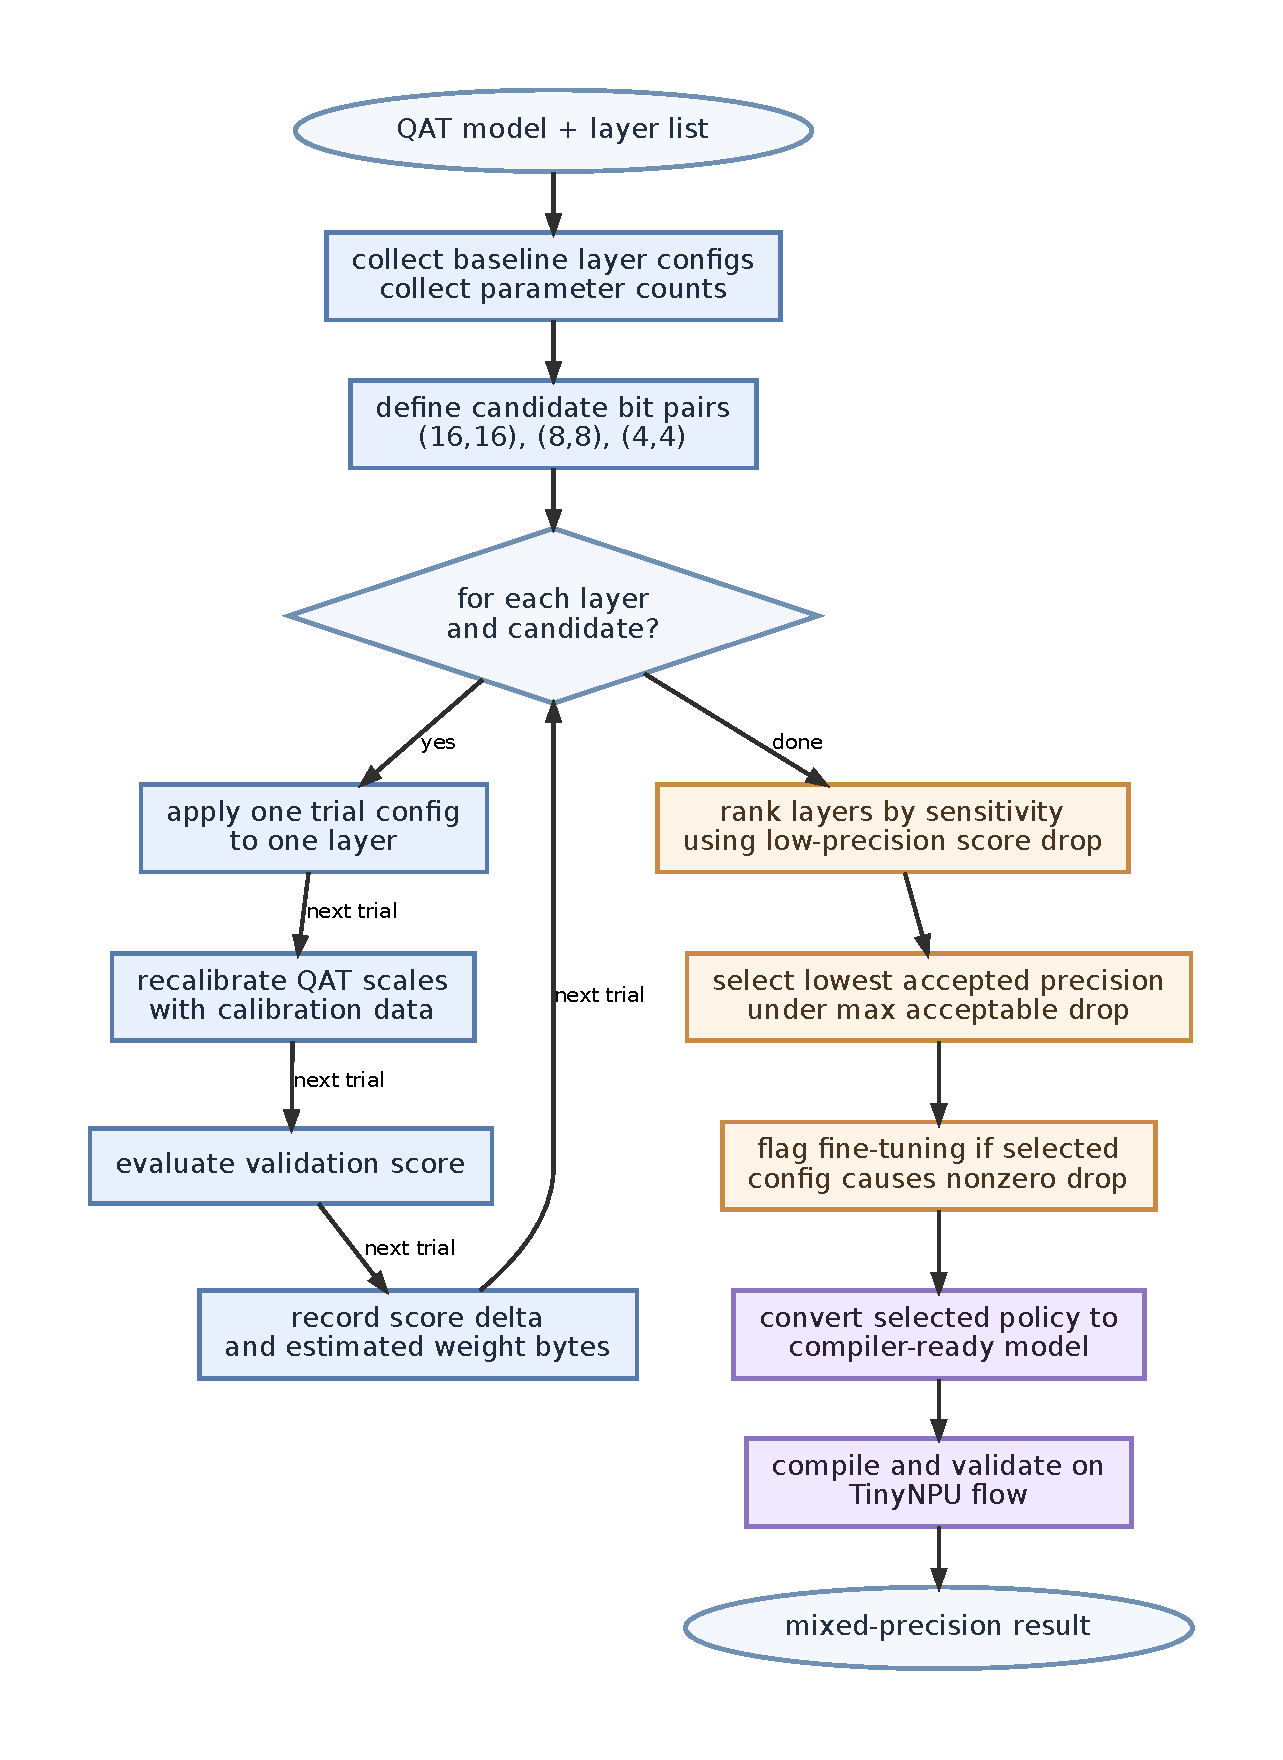
\includegraphics[width=0.88\textwidth,height=0.62\textheight,keepaspectratio]{diagrams/bit_selection_flow_graphviz.pdf}
    \caption{Heuristic mixed-precision selection flow used to obtain compiler-ready model variants.}
    \label{fig:bit-selection}
\end{figure}

The role of this subsystem is to bridge trained or quantized models into forms that the TinyNPU compiler can lower without losing track of numerical meaning. It supplies the weights, scales, multipliers, and shifts used in later RTL measurements.

\subsection{Structural Model}

\subsubsection{Accelerator Hardware}
The TinyNPU hardware is organized around a control path and a compute path. The control path sequences instructions and services the local control interface. The compute path consists of the unified buffer, streamer logic, a parameterized $N \times N$ output-stationary systolic array, and the post-processing unit.

The baseline local control contract is MMIO. Through this command path, the CV32E40P firmware can launch execution, read status, and transfer memory payloads one accelerator word at a time. That path is portable because it only assumes the standard control registers are present.

When the integration provides it, the same UB and IM storage can also be exposed through a wider shared-buffer window. This path is faster because it bypasses the MMIO memory-service loop for bulk preload and readback traffic. The arbitration policy is intentionally simple: it is time-multiplexed rather than fully concurrent. The firmware may use the shared window while the accelerator is idle, and shared access is blocked while the accelerator is busy. This avoids adding a more complex concurrent memory arbiter while still capturing the main performance benefit of direct buffer access.

\begin{figure}[H]
    \centering
    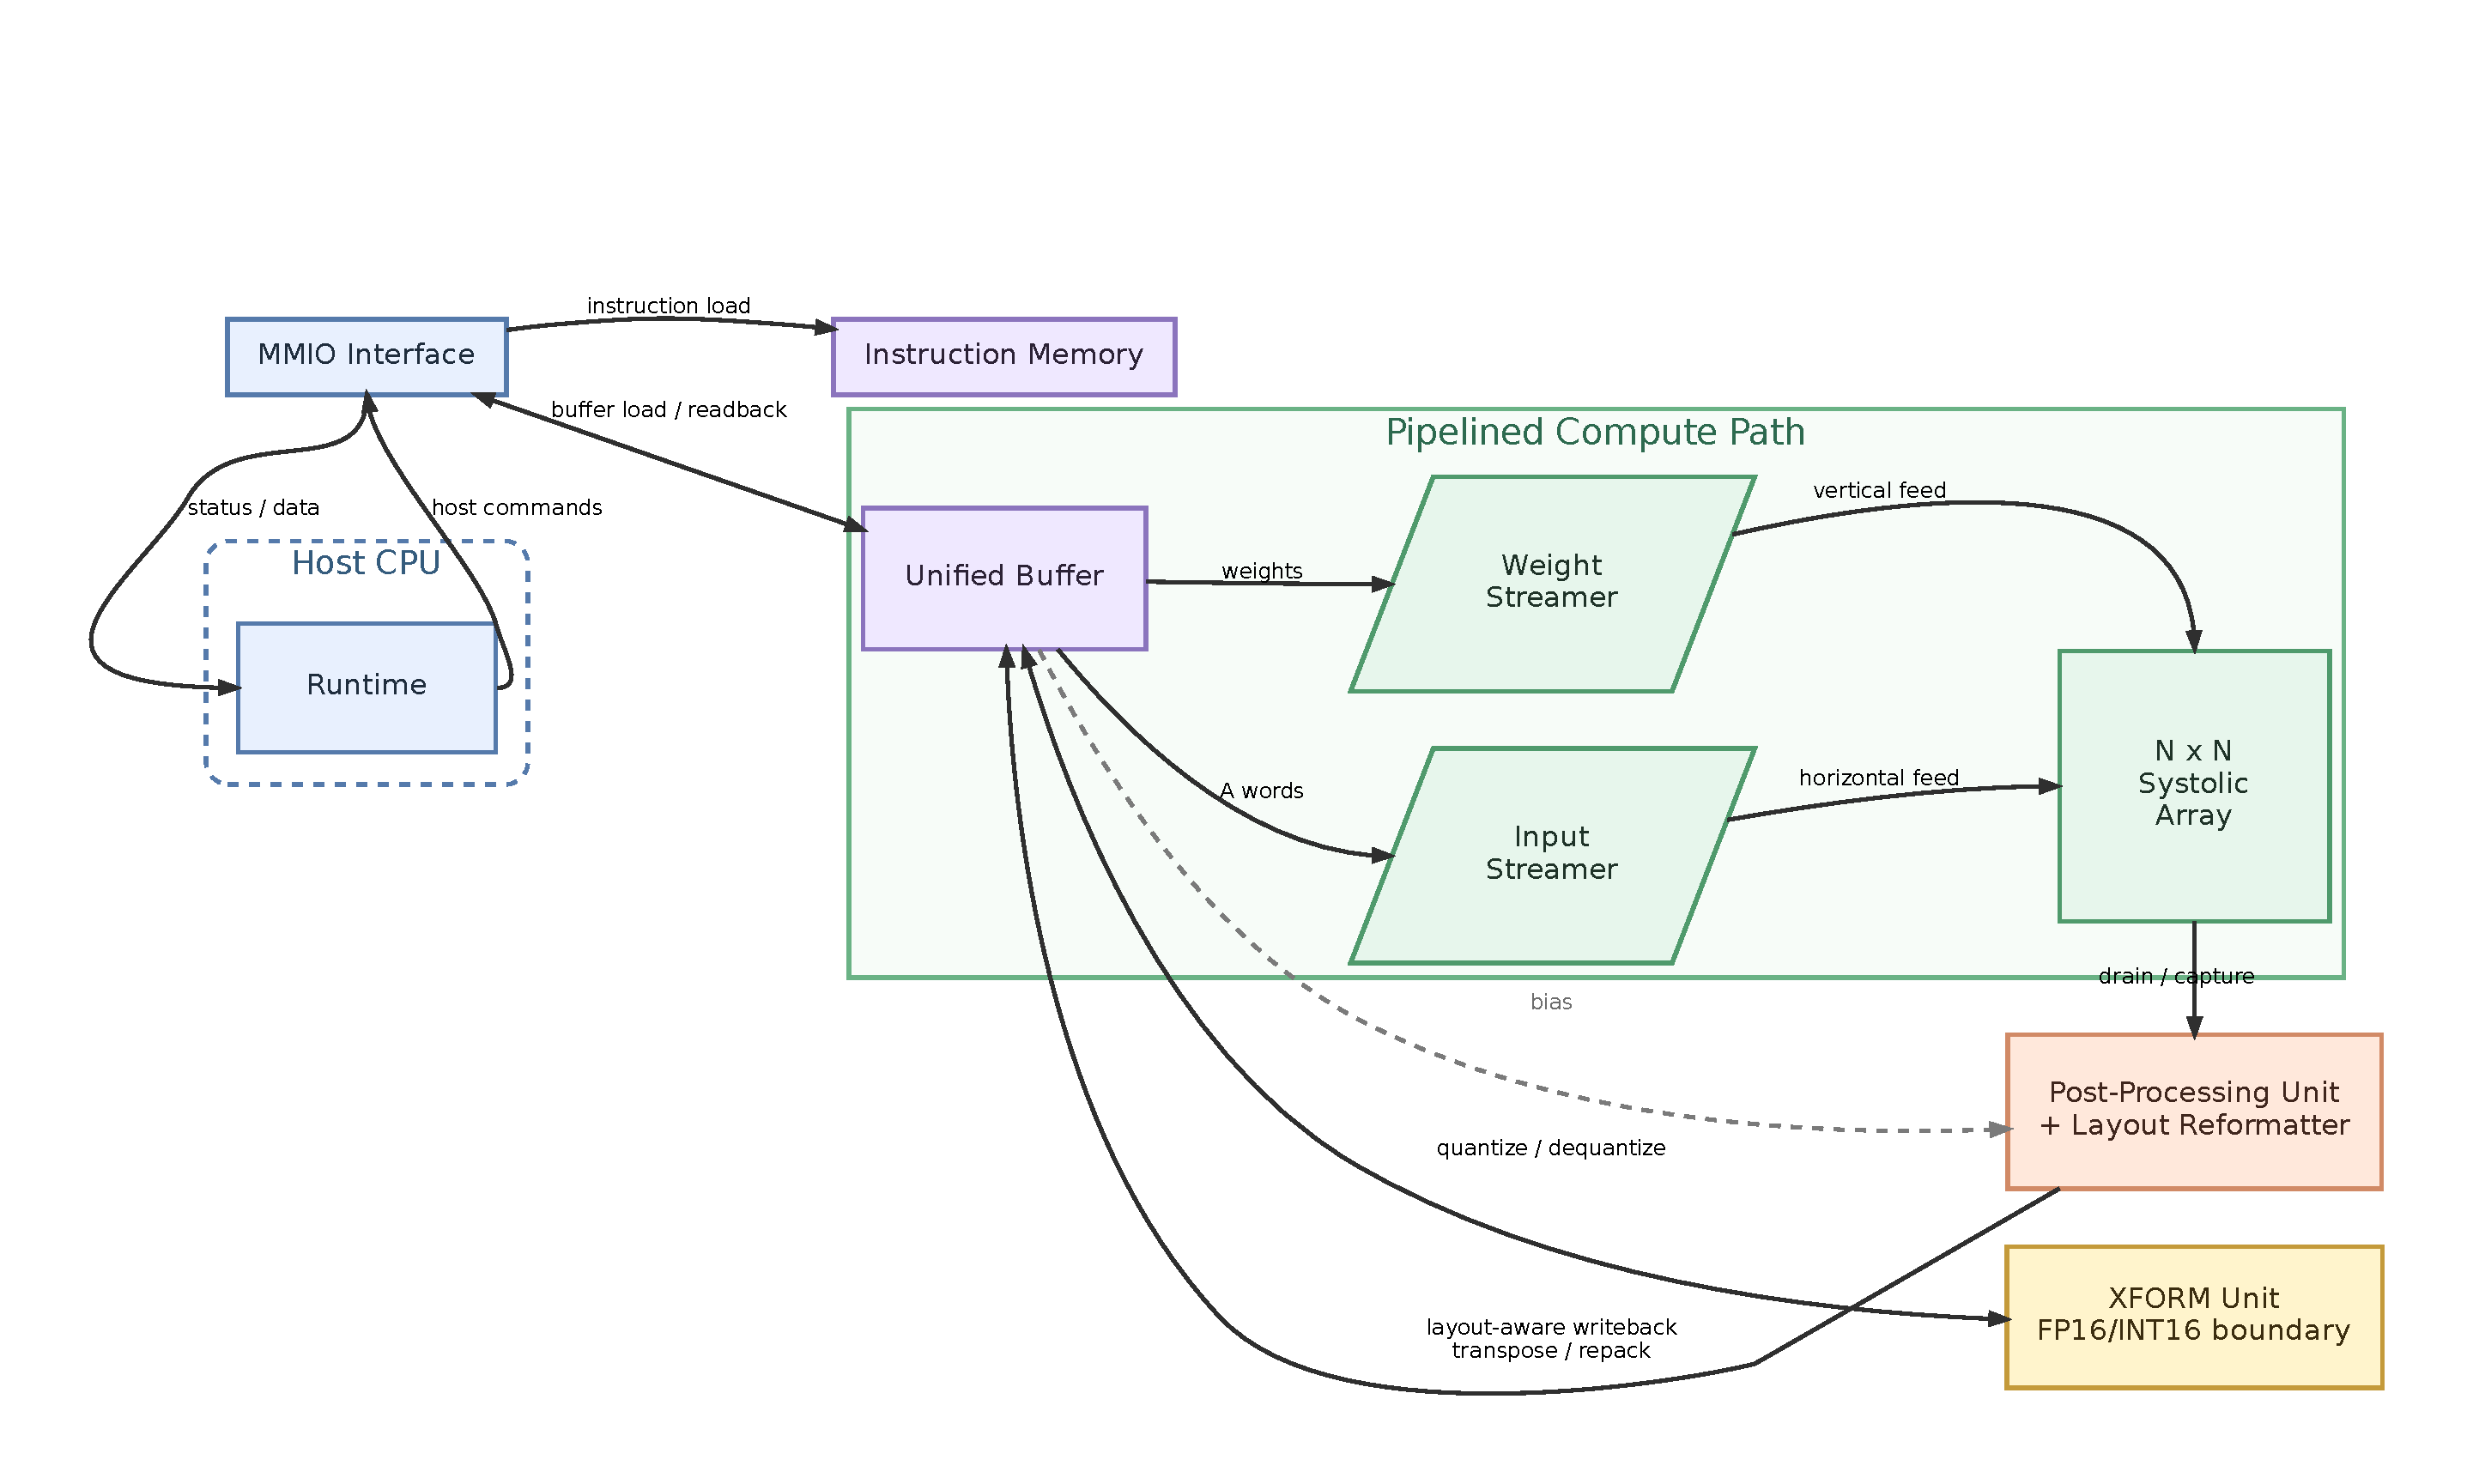
\includegraphics[width=\textwidth]{diagrams/hardware_architecture_graphviz.pdf}
    \caption{Top-level TinyNPU hardware architecture.}
    \label{fig:hardware-architecture}
\end{figure}

Figure~\ref{fig:hardware-architecture} shows the top-level organization. The compute path is a matrix path: the unified buffer feeds activation and weight streamers, the streamers feed the systolic array, and drained accumulators pass through the PPU before returning to the buffer. The figure also shows the two local access paths used by firmware. MMIO is the universal command and memory-service interface, while the shared-buffer window is the faster bulk path used for instruction images, tensor preload, and readback when the accelerator is idle. Boundary quantization and dequantization are handled by the runtime/compiler contract rather than by a separate hardware transform instruction.

\subsubsection{Systolic Array and Processing Element}
The array is output-stationary: packed activation words enter from the left edge and move one PE to the right per cycle, packed weight words enter from the top edge and move one PE downward per cycle, and each PE keeps its output accumulator stationary for the full reduction along the $K$ dimension. Only after the last $K$ contribution has been consumed does the array switch into drain mode and shift those accumulated results downward into the post-processing unit. This choice fits the dominant tiled-GEMM workload well because it keeps the reduction local to the PE and avoids repeatedly moving partial sums through the buffer system during the $K$ loop.

The streamer logic between the unified buffer and the array provides the timing skew that makes the systolic wavefront legal. On the activation side, row \(i\) is delayed before it enters the left edge; on the weight side, column \(j\) is delayed before it enters the top edge. The values themselves do not change. What changes is when they enter the array. That timing offset creates the diagonal wavefront expected by the schedule, so the activation and weight pieces that belong together meet at the correct PE in the correct cycle. A tile therefore executes in three phases: feed the packed $K$-steps into the array, allow the wavefront to fill across the remaining diagonals, and then drain the stationary accumulators.

The processing element is where mixed precision becomes concrete. Each PE consumes one packed activation word and one packed weight word. In INT16 mode that produces one signed multiply, in INT8 mode two byte multiplies, and in INT4 mode four nibble multiplies. The products are summed and accumulated into a 64-bit stationary register.

One practical implementation detail is that the vertical PE-to-PE link is wider than the packed weight word used during feed. The reason is reuse. During the compute phase the array only needs the packed incoming weight value, but during drain the same physical column path is reused to move full accumulators toward the PPU. Reusing one wider column link keeps the PE interface uniform across compute and drain instead of introducing a second dedicated drain network.

\begin{figure}[H]
    \centering
    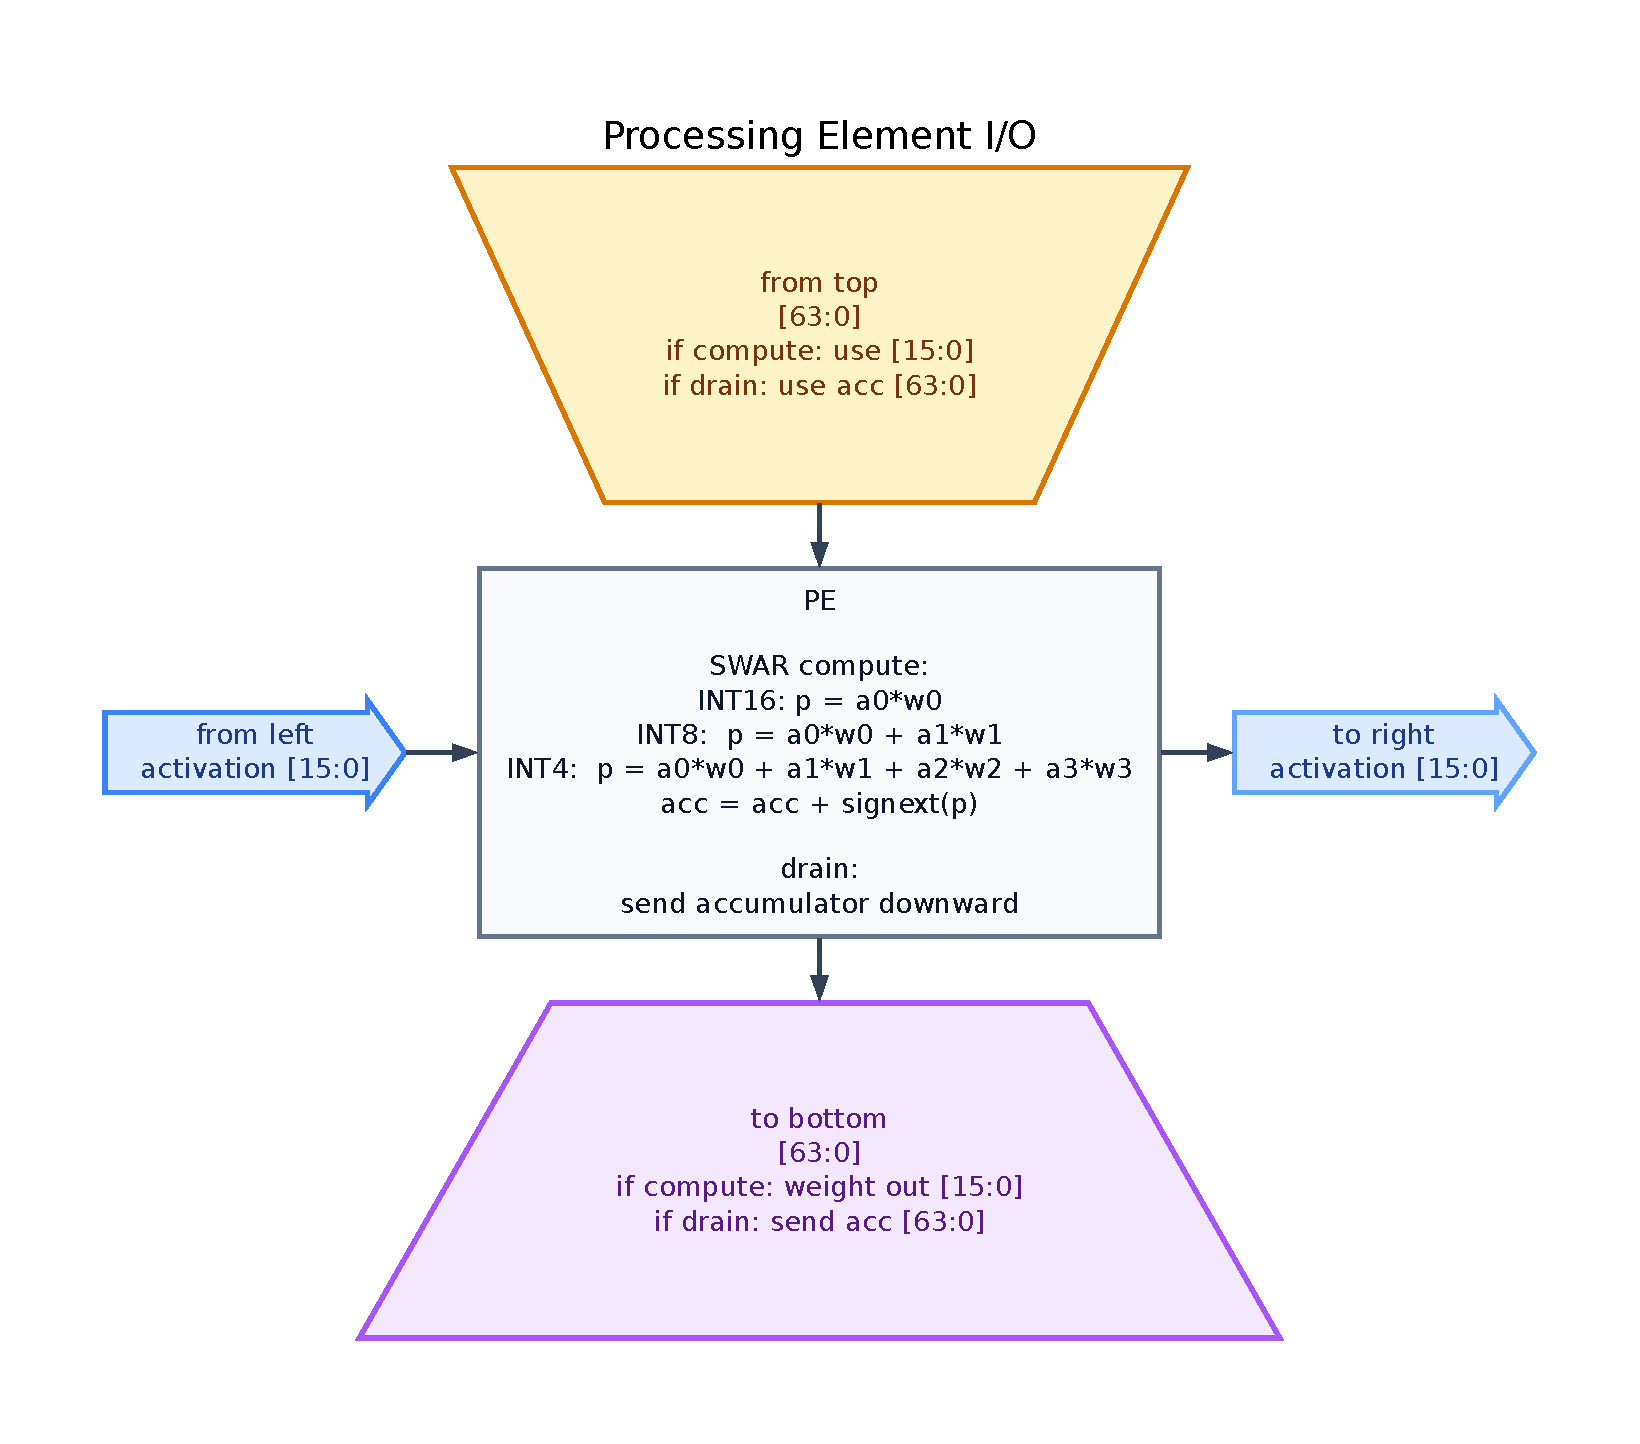
\includegraphics[width=0.88\textwidth,height=0.64\textheight,keepaspectratio]{diagrams/pe_internals_graphviz.pdf}
    \caption{Processing-element I/O in compute and drain modes.}
    \label{fig:pe-internals}
\end{figure}

\subsubsection{Post-Processing Unit}
The post-processing unit (PPU) is an \(N\)-lane row processor backed by an internal \(N \times N\) tile buffer. During drain, it receives one accumulator row vector per cycle from the bottom of the systolic array, processes the row in parallel, and stores the quantized result into its internal buffer. After the full tile has been captured, it writes the buffered rows back to the unified buffer.

The PPU is a sequenced pipeline, not a single combinational tail after the array. Drain capture, bias/rescale/activation, packed-lane formation, and unified-buffer writeback are separated into controlled phases. The control unit stalls the surrounding execution state until the PPU reports completion, so the architectural result is still one completed matmul tile even though the post-processing work spans multiple cycles internally. This staging is important for timing because the original operation combines wide accumulation, fixed-point rescale, activation selection, saturation, and packed writeback.

Before drain begins, the PPU loads the 32-bit bias vector for the output columns. For each drained row it then evaluates the same requantization pipeline lane by lane:
\[
\begin{aligned}
v &= (acc+bias)\times multiplier,\\
u &=
\begin{cases}
\mathrm{sat}_{16}(v), & shift = 0,\\
\mathrm{sat}_{16}\left((v + 2^{shift-1}) \gg shift\right), & shift > 0,
\end{cases}
\\
q &= \mathrm{clip}_{p}\left(\mathrm{act}(u)\right)
\end{aligned}
\]
where \(acc\) is the 64-bit drained accumulator, \(bias\) is a sign-extended 32-bit bias term, \(multiplier\) is the 16-bit fixed-point requantization factor, \(\gg\) is an arithmetic right shift, \(\mathrm{act}(\cdot)\) selects the configured post-processing nonlinearity, and \(\mathrm{clip}_{p}(\cdot)\) saturates to the signed range of the selected output precision. The PE and drain paths carry 64-bit accumulators; inside the staged PPU, the bias-added value is clamped into the narrower internal activation datapath before fixed-point multiplication. The compiler enforces the hardware ABI for this path: matmul rescale shifts are limited to 0--63, and activation-domain shifts for the hard-sigmoid gate and hard-GELU are limited to 0--15. These limits keep the variable-shift hardware bounded and make the quantization configuration part of the compile-time validity check. The activation stage supports plain ReLU, a MobileNetV3-style clipped affine gate used as the standalone hard-sigmoid output, and a hardware-friendly hard-GELU approximation. The hard-GELU path combines the GELU approximation \(x\cdot\sigma(1.702x)\) with the MobileNetV3-style hard gate \(x\cdot\mathrm{ReLU6}(\cdot+3)/6\), replacing the sigmoid with a clipped affine gate in the integer activation domain \cite{hendrycks2016gelu,howard2019mobilenetv3,kim2021ibert}. Concretely, the datapath performs bias addition, fixed-point multiplication, round-to-nearest when \(shift > 0\), the selected activation, and final saturation to INT16, INT8, or INT4.

Writeback is also precision-dependent. After the tile buffer has been filled, the ordinary C-layout path emits one buffered row per writeback cycle. For INT16 output, each 16-bit lane is written back directly. For INT8 and INT4 output, the PPU shifts the quantized value into the byte or nibble slot selected by the packed write offset, and the unified buffer applies a bit mask so that only that subword is written while sibling tiles in the same physical word are preserved. The control unit derives this packed write offset from the output tile index: two logical M-tiles share one physical word for INT8, and four logical M-tiles share one physical word for INT4.

The PPU therefore supports several practical writeback forms. For firmware-visible outputs it emits the ordinary C-oriented packed result layout. For internal chained tensors it can instead emit an A-compatible layout so the next accelerator consumer can read the result directly without a scalar layout conversion on the core. The RTL also contains INT16 K-cache and V-cache append modes for transformer-shaped experiments. In the Llama-like lowering, V-cache append can be selected directly after the V projection. K-cache update is different because RoPE is always executed on the core in this design, and the rotated key is what must be stored. Appending the unrotated key directly from the accelerator would force firmware to read that cache entry back, apply RoPE, and rewrite the same cache location through the shared buffer. That round trip defeats the purpose of the append mode, so the compiler keeps the Llama-like K-cache update as an explicit scalar cache step after RoPE. The compiler selects the required form when it lowers a segment.

\subsubsection{Compiler}
The compiler converts model structure into a mixed execution structure. Rather than generating a monolithic accelerator-only program, it constructs an \texttt{ExecutionPlan} whose steps are typed as \texttt{NpuSegment}, \texttt{ScalarOp}, or \texttt{VerifyTensor}. A scalar operation is owned by the CV32E40P core: it is part of the compiled plan, but it is not executed by the matrix accelerator. This keeps unsupported behavior and verification points explicit instead of hiding them inside an accelerator-only view.

The Python-side intermediate representation has two layers. The first layer records tensors with shape, dtype, storage role, and metadata such as cache role or view relationship. The second layer records operations and execution steps. Matmul-like operations carry the operands, bias tensor, precision, rescale multiplier and shift, activation selector, and required output layout. Scalar operations represent work intentionally executed on the core, such as normalization, softmax, reshape, cache scatter, or verification. This representation is semantic enough for partitioning and validation, but still close enough to the hardware contract that lowering can emit exact instruction fields and buffer layouts.

\subsubsection{Runtime and Verification}
The deployed firmware runtime is linked into the generated CV32E40P program. It executes the compiled plan as a mixed core/accelerator loop. For each step, it either launches an accelerator segment, executes a required scalar operation on the core, or checks an expected tensor. Scalar core work is therefore visible both in the plan and in the benchmark accounting.

Verification is built into this same path. Compiler-owned expected tensors can be checked during execution, and the runtime can record RTL cycle counts for accelerator run windows separately from software-side overhead.

\subsection{Dynamic Model}

\subsubsection{Compilation Flow}
Listing~\ref{lst:compiler-ir-example} shows the two practical ways to enter the compiler. A model can come from a small quantized PyTorch module, or it can be assembled directly with the IR builder when the workload is already known at the tensor/operation level. The compiler does not require the whole model to be accelerator-supported. It lowers the legal matrix regions into accelerator segments and keeps the remaining operations as explicit scalar operations owned by the core.

\begin{lstlisting}[language=Python,caption={Example PyTorch input and equivalent IR-builder construction.},label={lst:compiler-ir-example}]
# PyTorch-side structure accepted by the frontend
class TinyMlp(nn.Module):
    def forward(self, x):
        h = torch.relu(self.fc0(x))   # Linear + bias + ReLU
        return self.fc1(h)            # Linear + bias

# Direct IR-builder path for the same kind of lowered workload
b = IRBuilder()
b.tensor("x", (1, 784), DType.INT16, TensorKind.INPUT)
b.constant("w0", w0_i16, DType.INT16)
b.constant("b0", b0_i32, DType.INT32)
b.intermediate("h", (1, 256), DType.INT16)
fc0 = b.matmul("fc0", "x", "w0", "h", bias="b0",
               activation="relu", out_layout="A")
b.segment("seg0", ops=[fc0], inputs=["x", "w0"], outputs=["h"])
b.output("y", (1, 10), DType.INT16, is_final_output=True)
b.verify("y")
plan = b.finalize(inputs=["x"], outputs=["y"])
\end{lstlisting}

\begin{figure}[H]
    \centering
    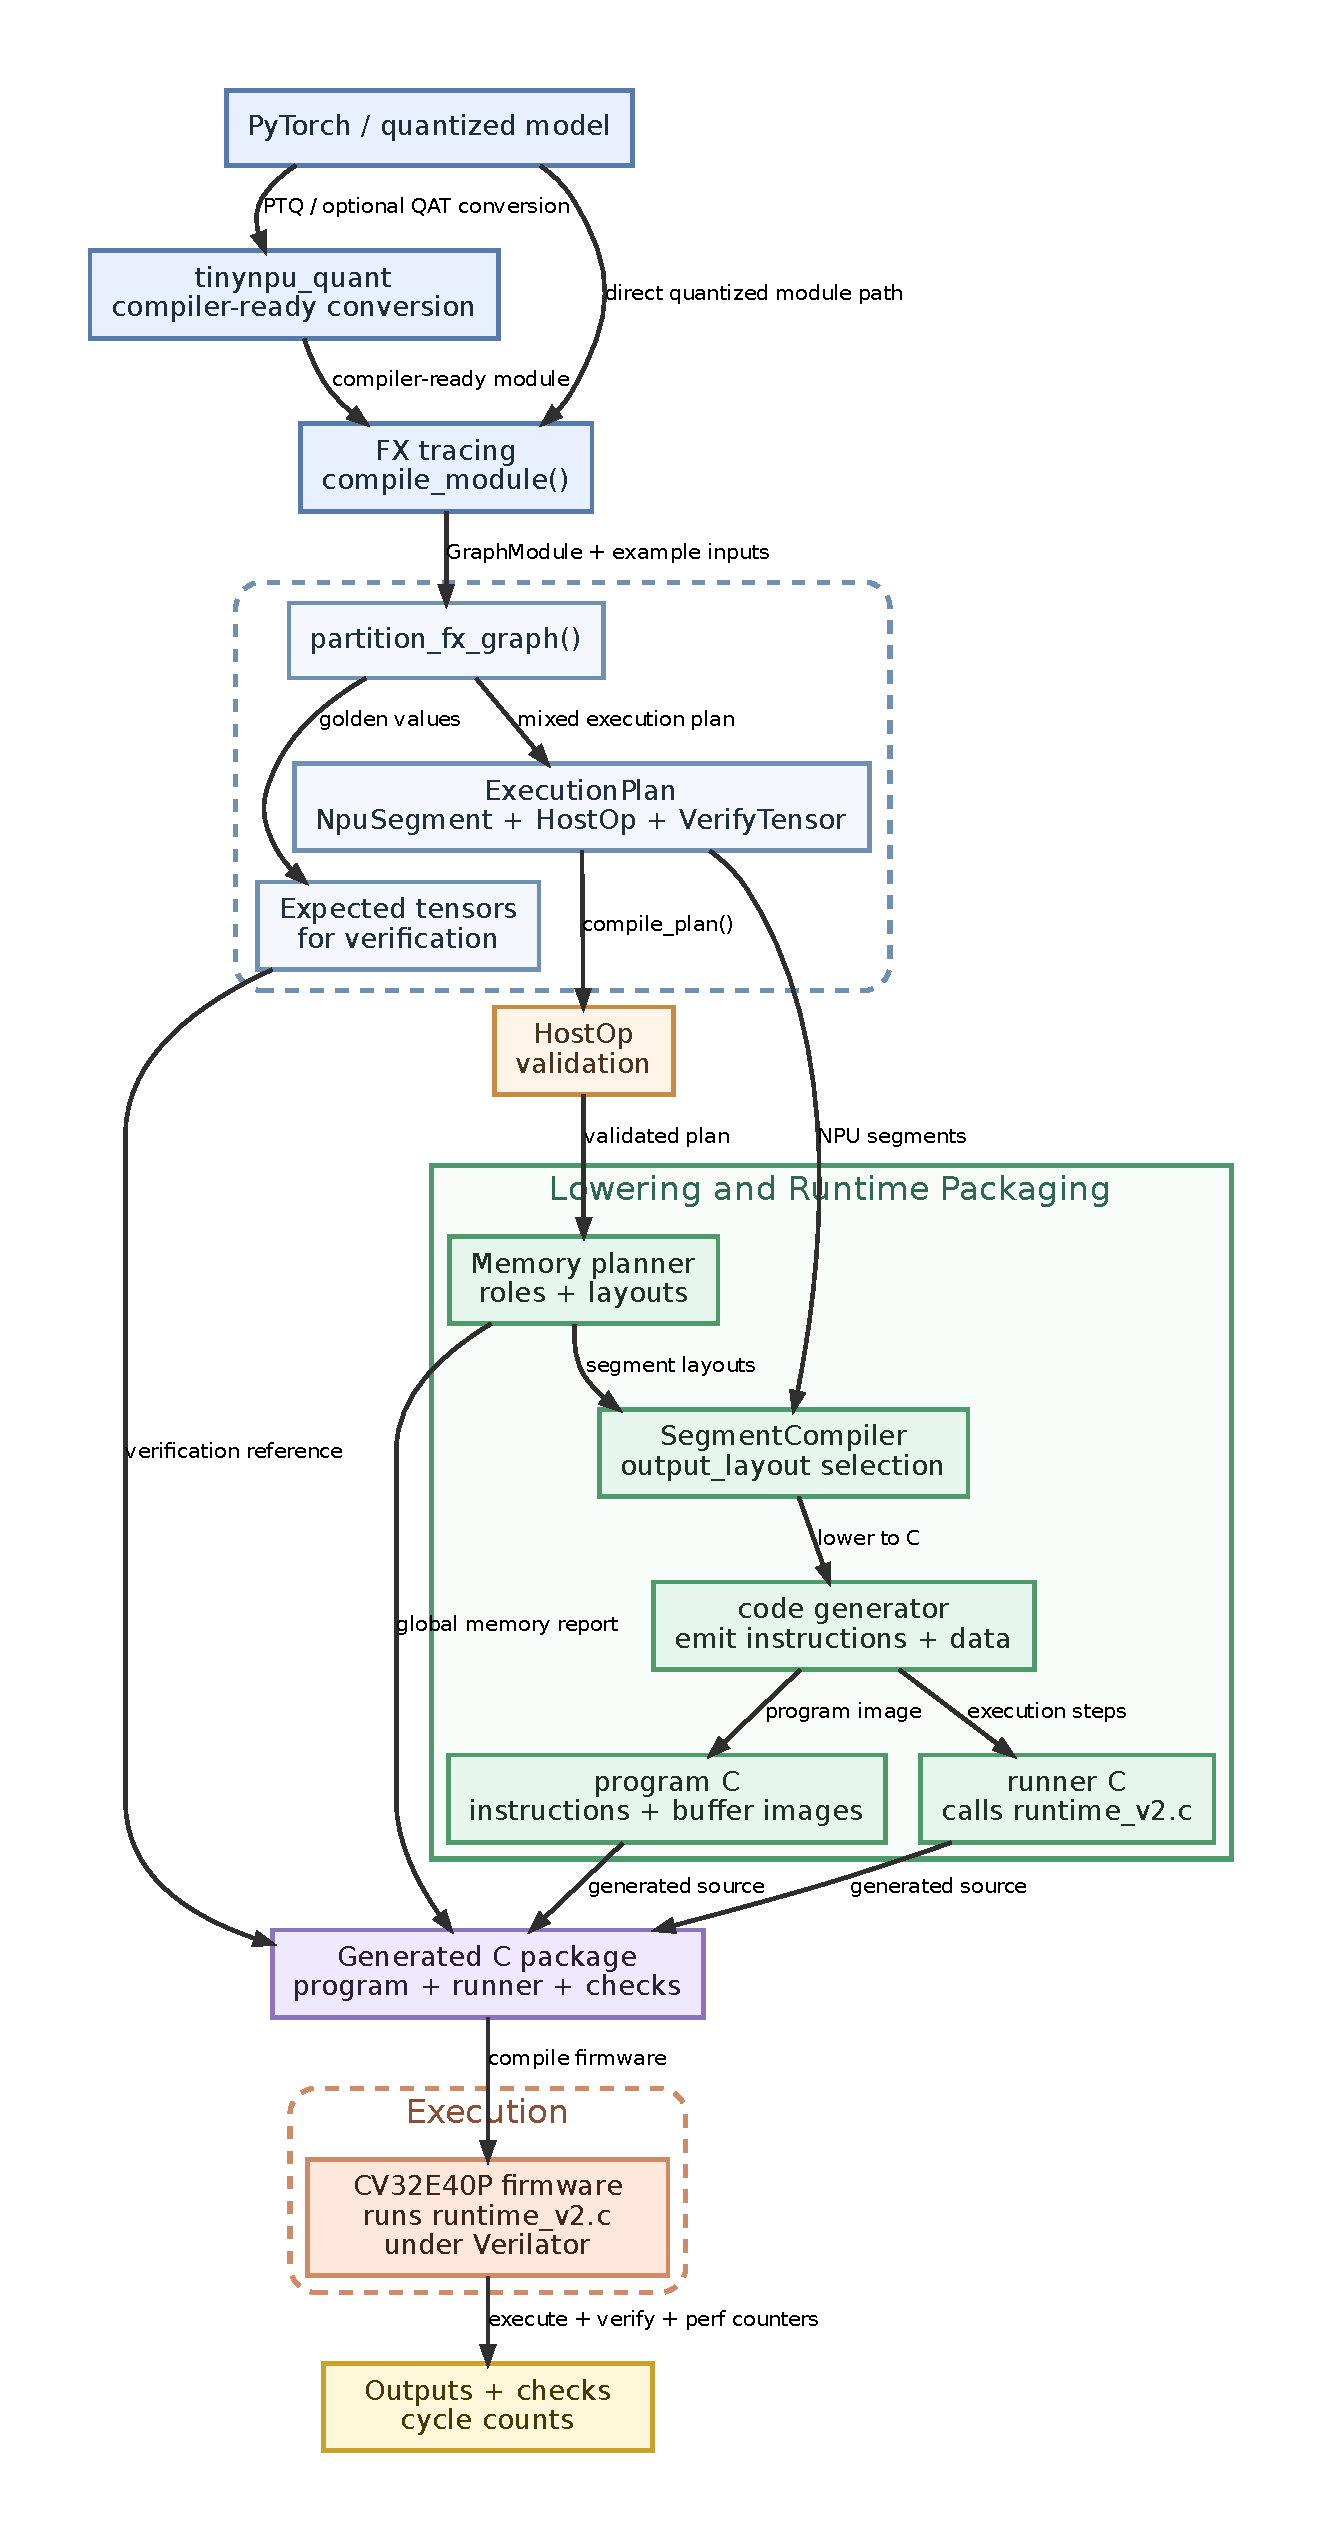
\includegraphics[width=0.92\textwidth,height=0.72\textheight,keepaspectratio]{diagrams/compiler_stack_graphviz.pdf}
    \caption{Compiler and firmware flow used to execute a TinyNPU artifact.}
    \label{fig:compiler-stack}
\end{figure}

Figure~\ref{fig:compiler-stack} summarizes the software flow. A model enters either as a supported quantized PyTorch module, through a compiler-ready conversion path, or through the direct IR-builder path shown in Listing~\ref{lst:compiler-ir-example}. The IR-builder route enters at the same execution-plan level as the traced frontend. From that point onward, the compiler partitions the plan, validates scalar operations, lowers each accelerator segment through memory planning and segment lowering, and emits the C data structures used by firmware.

Packing is part of the compiler contract as well. The backend uses role-specific physical layouts for activation-side tensors, weight-side tensors, output buffers, and bias payloads. These are physical storage forms rather than semantic tensor meanings, but they are essential because legal execution depends on matching memory layout to the real feed directions and writeback format of the accelerator. The compiler annotates the required physical output layout explicitly, and the emitted instruction stream carries that selection into the RTL writeback path.

The compiler is responsible for more than emitting instruction fields. It decides where accelerator regions begin and end, which tensors must be resident in the unified buffer, which outputs need an accelerator-consumable layout, and which operations remain on the core. The partitioner emits a mixed execution plan and inserts a segment boundary whenever execution must return to firmware, a verification point is requested, or an operation is outside the supported accelerator contract. As a result, scalar work such as dequantization, softmax, mean, layout restoration, and verification is represented directly as \texttt{ScalarOp} or \texttt{VerifyTensor} steps rather than being buried inside an accelerator launch.

Memory planning makes those execution boundaries explicit in the buffer layout. The unified buffer is divided into a static zone and a dynamic zone: weights and biases receive globally assigned packed addresses that can be shared across segments, while activations and outputs are placed in a per-segment dynamic region with liveness-based reuse. The planner also treats layout as a real physical requirement. If a tensor must be emitted in an A-compatible layout for an internal chained consumer, that requirement is carried explicitly instead of being inferred informally.

\subsubsection{Runtime Execution Flow}
The generated program is therefore closer to a small bytecode interpreter than to a hand-written benchmark. The compiler emits constant C tables into the program image: tensor descriptors, unified-buffer preload images, instruction-memory preload images, accelerator segment descriptors, scalar-operation descriptors, verification descriptors, and a top-level operation list. At runtime, the firmware walks that operation list in order. Preload entries copy static tensor and instruction images into accelerator-visible memory. Segment entries stage live input tensors into the required physical layout, start the accelerator at the segment's instruction-memory address, wait for completion, and read selected outputs back into runtime tensors. Scalar-operation entries call the corresponding helper on the CV32E40P core, for example normalization, softmax, reshape, or cache update. Verification entries compare a runtime tensor against compiler-owned expected data.

This structure is important because it makes the execution boundary measurable. The accelerator instruction stream controls only the tiled matrix region inside one segment. The firmware schedule around it accounts for the work needed to make that segment usable in a full program: tensor binding, preload, staging, launch, readback, scalar core operations, and optional verification. The same runtime can therefore execute a pure scalar-core plan, a mostly accelerator-backed plan, or a mixed attention-style plan without changing the hardware interface.

The firmware runtime also owns repeated-run behavior. It can preserve reusable state such as static unified-buffer contents and preloaded instruction-memory images across runs.

\begin{figure}[H]
    \centering
    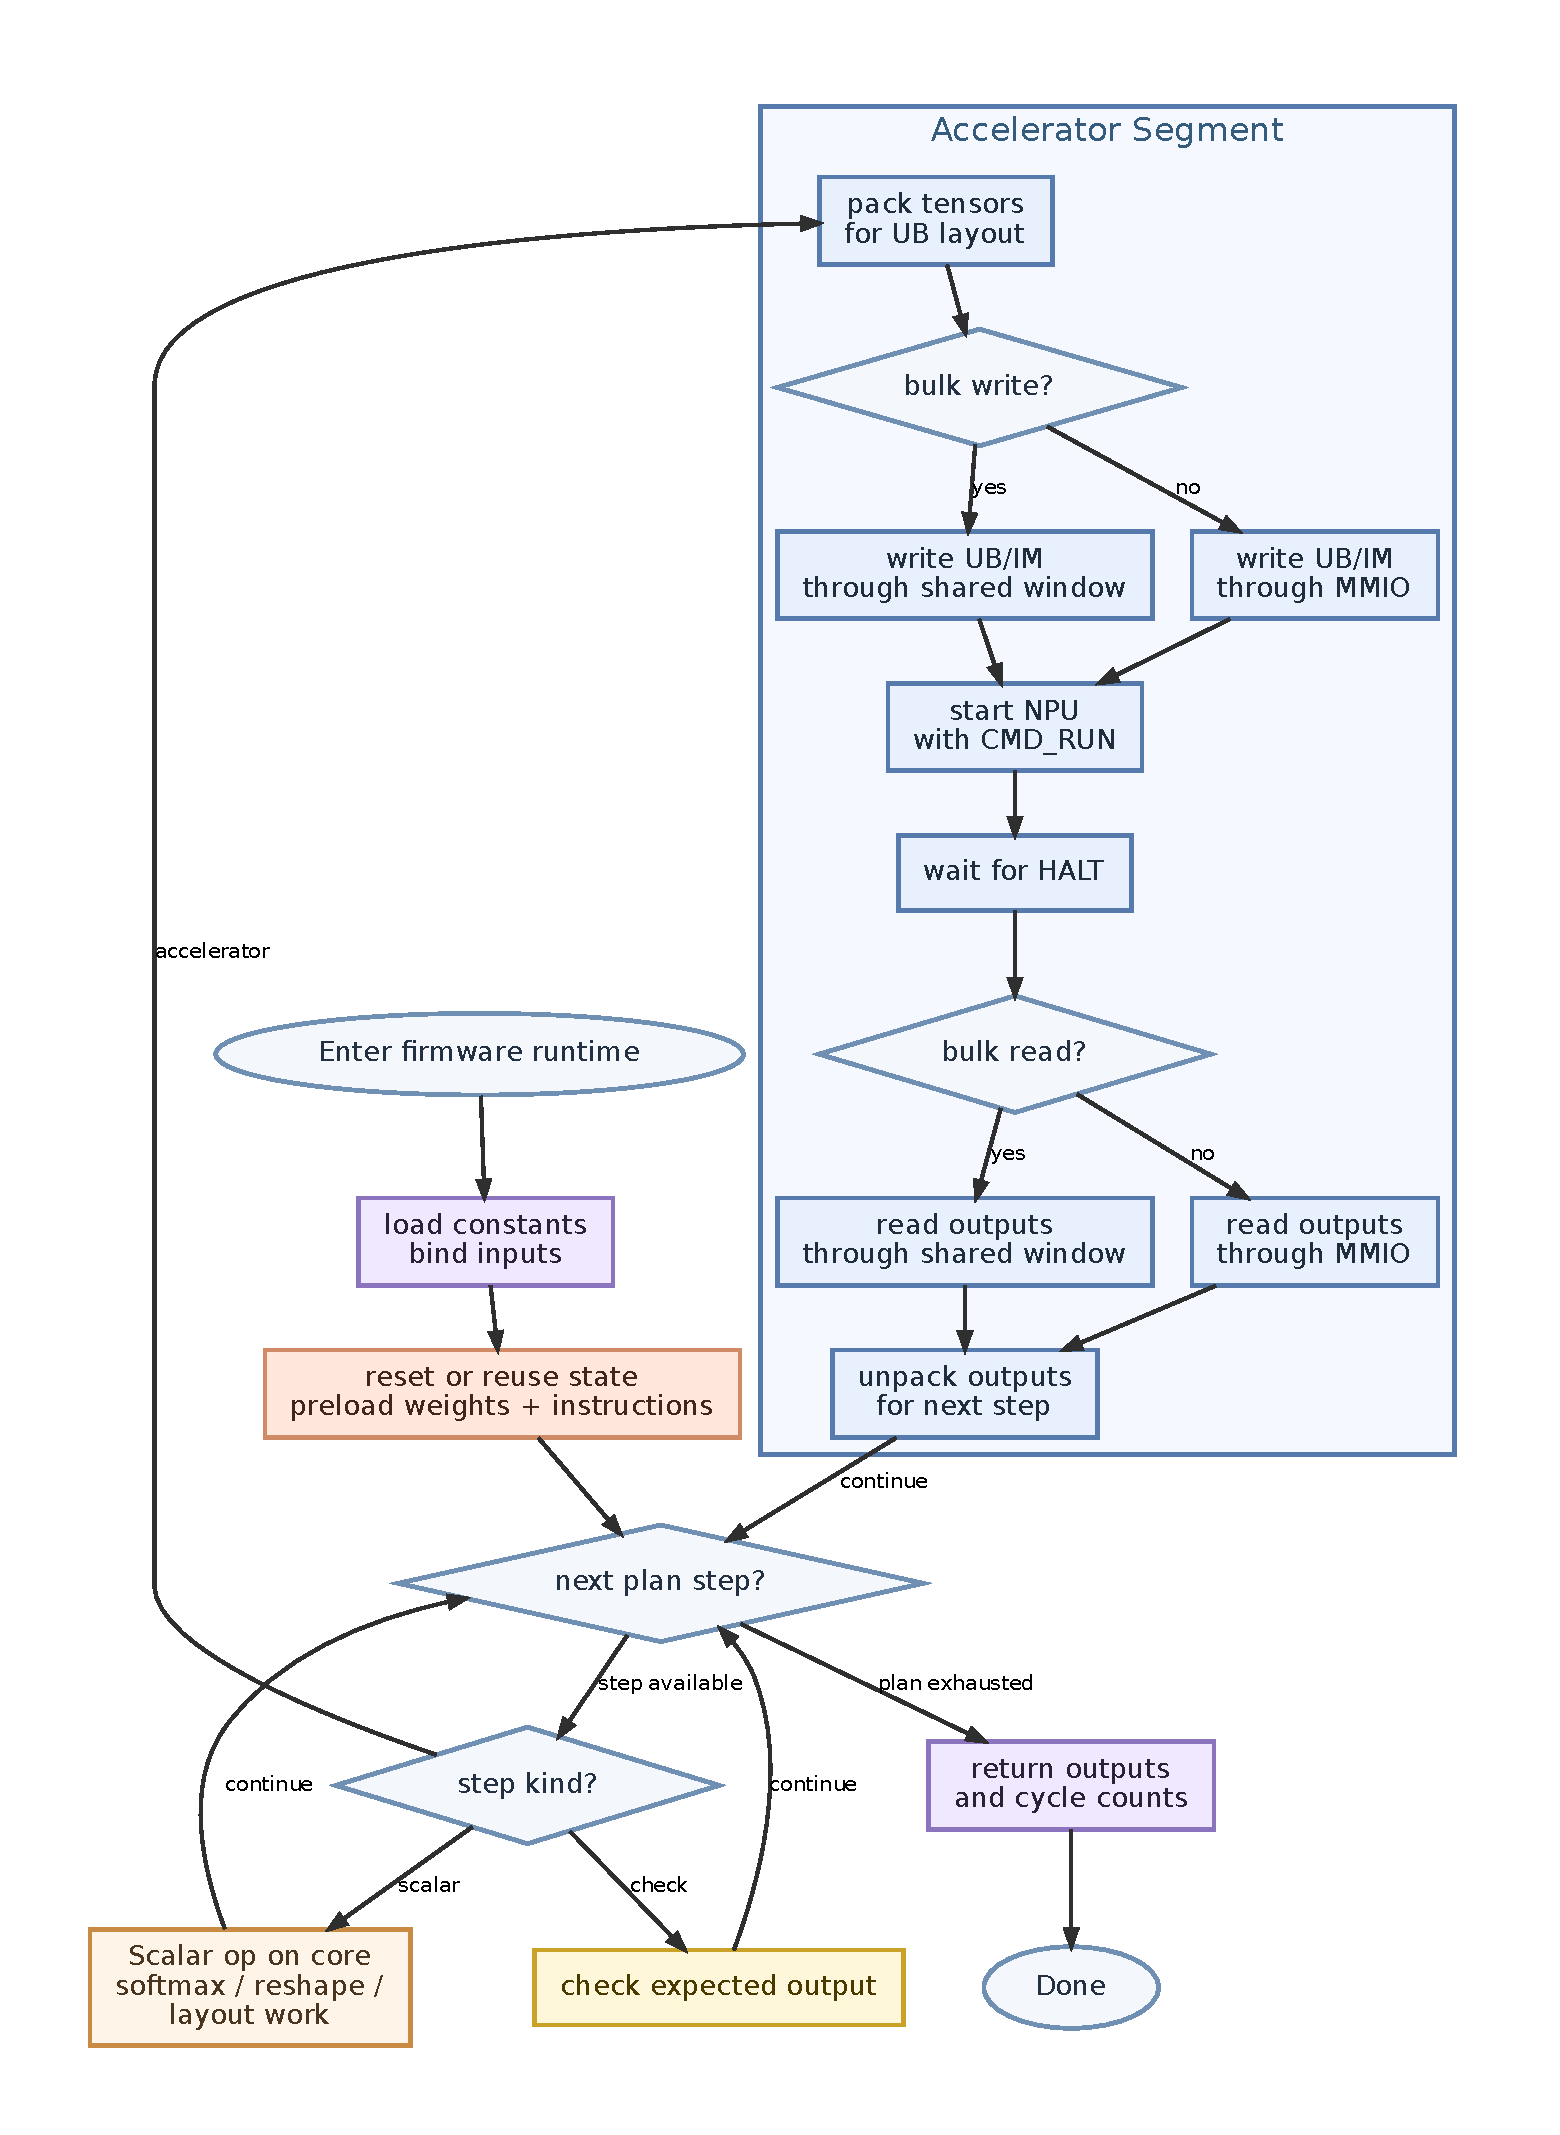
\includegraphics[width=0.9\textwidth,height=0.58\textheight,keepaspectratio]{diagrams/runtime_state_graphviz.pdf}
    \caption{Firmware runtime flow for executing a compiled TinyNPU artifact.}
    \label{fig:runtime-state}
\end{figure}

Figure~\ref{fig:runtime-state} shows this firmware loop. For accelerator segments, the runtime packs logical tensors into the physical layouts expected by the datapath, stages data into the unified buffer and instruction memory, starts the accelerator, waits for completion, and reads the outputs back. Output-layout support lets chained internal tensors be written directly in the layout needed by the next accelerator consumer.

\subsubsection{Transformer Block Execution}
The transformer experiments use reduced-dimensional decoder blocks rather than full pretrained language models. Their purpose is to stress the compiler/runtime boundary on attention-shaped workloads: normalization, attention score formation, softmax, key/value cache handling, residual connections, and feed-forward sublayers. These blocks are therefore structural tests of the system contract, not language-quality benchmarks.

The Llama-like block uses RMSNorm, grouped-query attention, scalar RoPE on Q/K, an attention output projection, and a SwiGLU feed-forward tail. Dense projections are lowered to INT16 accelerator matmuls: Q/K/V projection, QK score matmul, probability-times-value matmul, attention output projection, gate/up projections, and down projection. The core handles the non-matrix pieces: RMSNorm, RoPE, softmax, residual adds, SiLU, elementwise feed-forward multiplication, and the quantize/dequantize boundaries around those operations.

Prefill and decode exercise different cache behavior. In prefill, the prompt is processed as a short sequence and the key/value cache is materialized for all prompt positions. In decode, the input has one new token, the previous cache is reused, and attention reads over the prompt plus the new token. The RTL includes INT16 cache append and cache-read modes. V-cache append can be used directly after the V projection. K-cache append is only directly usable when the value being written is already the rotated key; because this design keeps RoPE on the core, the Llama-like K-cache update remains a scalar cache update after RoPE.

The GPT-2-like block uses LayerNorm, causal self-attention, an attention output projection, residual connections, and a two-layer GELU feed-forward network. Its accelerator work is the same class of dense matmul work: Q/K/V projections, score and value matmuls, output projection, and feed-forward projections. The core handles LayerNorm, causal mask and softmax, residual adds, and cache bookkeeping. The reported GPT-2-like runtime experiment chains two blocks back-to-back and includes prefill, decode, and cache reuse so that intermediate state must survive across more than one block.

\begin{table}[H]
    \centering
    \footnotesize
    \caption{Transformer-like block lowering boundary. The blocks are reduced-size structural tests, not full pretrained GPT-2 or Llama models.}
    \label{tab:transformer-lowering}
    \begin{tabularx}{\textwidth}{|l|>{\raggedright\arraybackslash}X|>{\raggedright\arraybackslash}X|}
        \hline
        \textbf{Block} & \textbf{Accelerator work} & \textbf{Core/runtime work} \\
        \hline
        Llama-like & INT16 Q/K/V projections, attention score matmul, probability-times-value matmul, attention output projection, gate/up projections, down projection & RMSNorm, scalar RoPE, softmax, residual adds, SiLU and elementwise feed-forward multiply, K-cache update after RoPE, V-cache append where legal, quantize/dequantize boundaries \\
        \hline
        GPT-2-like & INT16 Q/K/V projections, attention score matmul, probability-times-value matmul, attention output projection, feed-forward projections & LayerNorm, causal mask and softmax, residual adds, cache reuse across prefill and decode, quantize/dequantize boundaries \\
        \hline
    \end{tabularx}
\end{table}

\subsection{Scope Boundaries}
The system targets a narrow but concrete contract. The software stack is best understood as a chain of APIs and scripts that produce legal, benchmarkable inputs for the accelerator: train or load a small model, assign quantization parameters, build a mixed execution plan, emit firmware data structures, and run the result in RTL. It is not intended to solve global mixed-precision search, optimal scale assignment, or automatic lowering for arbitrary neural networks.

This boundary is intentional. The compiler supports a bounded operator set and routes remaining work through explicit scalar operations on the core. The evaluation therefore focuses on trained MNIST-derived models, controlled kernel benchmarks, and small transformer-like blocks. Those workloads are sufficient to study the interaction between architecture, compilation, runtime overhead, and timing closure without overstating workload coverage.

\newpage
\section{Evaluation Setup}
All reported performance numbers come from the CV32E40P example testbench with TinyNPU attached in Verilator. In this report, \emph{TinyNPU} refers to the full local system: the CV32E40P firmware core, the accelerator datapath, the local memories, and the runtime contract between them. The word \emph{core} refers to the CV32E40P scalar processor. The word \emph{accelerator} or \emph{NPU} refers to the matrix hardware: unified buffer, streamers, systolic array, control path, and post-processing unit. In this prototype, the core has two roles: it executes scalar model operations, and it also performs local orchestration. A larger deployment could keep the core as the scalar companion while moving higher-level scheduling to an external host or SoC control processor.

The core controls the accelerator through MMIO command and status registers. The integration also provides a shared-buffer window for unified-buffer and instruction-memory traffic. In this setup the shared window is an idle-time preload and readback path: firmware uses it while the accelerator is idle, then execution transfers ownership to the accelerator for the run itself.

The evaluation has three parts. First, controlled multi-tile GEMM benchmarks measure end-to-end MAC/cycle under the shared-buffer runtime path. Second, trained MLP and convolution models are compared against an external ONNX2C-generated core baseline and converted to wall-clock time using routed timing estimates. Third, reduced GPT/Llama-like blocks test whether attention-shaped execution improves as model dimensions grow.

ONNX2C is used as the independent core-only baseline. It converts an ONNX graph into plain C code, which is compiled into the CV32E40P firmware image and executed as FP32 code on the core/FPU without using the TinyNPU runtime or accelerator-resident buffers. This gives a stronger comparison than a hand-written local baseline because the reference path is generated by a separate toolchain.

Correctness for the measured runs comes from compiler-owned expected tensors, runtime verification, or \texttt{autoverify} checks when explicit verify steps are not emitted. Separate unit, regression, and cocotb tests are used during development, but the headline numbers in this section come from RTL execution of either the core-only ONNX2C baseline or the full TinyNPU system path.

Cycle measurements are taken around the work being compared. In the ONNX2C core baselines, the timer starts immediately before the generated model function is called and stops immediately after it returns; diagnostic printing happens after the measured window. In the TinyNPU accelerator path, segment, preload, scalar-operation, and repeated-run totals are accumulated from timer windows around the corresponding work and printed afterward. Print statements affect Verilator wall-clock runtime, but not the reported architectural cycle counts.

Wall-clock comparisons use the Vivado timing boundary. The core-only CV32E40P configuration routes at 66.0 MHz. The fitted integrated TinyNPU system with real BRAM routes at an estimated 49.00 MHz after place-and-route. Because the integrated system clocks below the core-only baseline, the accelerator path must save enough cycles to overcome a \(66.0/49.00 \approx 1.35\times\) clock-frequency disadvantage before it wins in wall-clock time.

\begin{table}[H]
    \centering
    \footnotesize
    \caption{Vivado timing boundary used for wall-clock comparisons. Target device is \texttt{xc7a200tsbg484-1}.}
    \label{tab:vivado-timing}
    \begin{tabularx}{\textwidth}{|l|c|c|c|Y|}
        \hline
        \textbf{Design} & \textbf{Target} & \textbf{WNS} & \textbf{Status} & \textbf{Use in report} \\
        \hline
        Core only & 66.0 MHz & 0.000 ns & Meets & ONNX2C/core wall-clock baseline. \\
        \hline
        Accelerator only, real BRAM & 50 MHz & +0.106 ns & Meets & Standalone accelerator timing with implemented memories. \\
        \hline
        TinyNPU system, fitted real BRAM & 50 MHz & -0.408 ns & Routed, below target & Integrated core+accelerator wall-clock estimate, 49.00 MHz. \\
        \hline
    \end{tabularx}
\end{table}

Table~\ref{tab:vivado-resource-utilization} reports post-route resource utilization for the same routed configurations. The standalone core is small compared with the accelerator. The integrated TinyNPU system is dominated by the accelerator memories and arithmetic datapath: block RAM usage reaches 74.52\% of the selected Artix-7 device, while LUT and DSP use remain below 40\% and 25\%, respectively.

\begin{table}[H]
    \centering
    \footnotesize
    \caption{Vivado post-route resource utilization for the timing configurations in Table~\ref{tab:vivado-timing}. Target device is \texttt{xc7a200tsbg484-1}.}
    \label{tab:vivado-resource-utilization}
    \resizebox{\textwidth}{!}{%
    \begin{tabular}{|l|r|r|r|r|}
        \hline
        \textbf{Design} & \makecell{\textbf{Slice}\\\textbf{LUTs}} & \makecell{\textbf{Slice}\\\textbf{Registers}} & \makecell{\textbf{Block RAM}\\\textbf{Tiles}} & \textbf{DSPs} \\
        \hline
        Core only & 4,521 (3.38\%) & 2,132 (0.80\%) & 0 (0.00\%) & 5 (0.68\%) \\
        \hline
        Accelerator only, real BRAM & 42,751 (31.95\%) & 18,252 (6.82\%) & 272 (74.52\%) & 172 (23.24\%) \\
        \hline
        TinyNPU system, fitted real BRAM & 49,180 (36.76\%) & 20,290 (7.58\%) & 272 (74.52\%) & 177 (23.92\%) \\
        \hline
    \end{tabular}}
\end{table}

The integrated timing point uses the BRAM-mapped TinyNPU configuration that fits the target FPGA. A direct rerun with the largest current unified-buffer default does not place on \texttt{xc7a200tsbg484-1}: Vivado reports 512 required RAMB36/FIFO cells against 365 available. This makes local memory capacity the main FPGA resource boundary for larger tensors; LUT and DSP utilization leave more headroom than the BRAM system. The reported wall-clock conversion therefore uses the fitted memory configuration rather than the oversized debug-capacity default.

\newpage
\section{Comparative Evaluation and Discussion}
This section focuses on artifacts that are representative of the implemented system: controlled GEMM scaling, trained-model wall-clock comparison, and small transformer-like block scaling. The main distinction is between inner-kernel capability and system-level behavior. A compute-only speedup is not enough if staging, scalar core operations, launch overhead, or a lower integrated clock dominate the full program.

In the following tables, cycle speedup compares architectural cycles directly. Wall speedup also applies the timing assumptions from Table~\ref{tab:vivado-timing}: 66.0 MHz for the ONNX2C core baseline and 49.00 MHz for the fitted TinyNPU system. The ONNX2C baseline has no accelerator-resident state, so it is reported as one function-call timing. The TinyNPU accelerator path has two useful measurement boundaries, summarized in Table~\ref{tab:cold-warm-boundary}.

\begin{table}[H]
    \centering
    \footnotesize
    \caption{Cold and warm TinyNPU accelerator-path measurement boundaries. Warm execution is a repeated-inference boundary, not a kernel-only boundary.}
    \label{tab:cold-warm-boundary}
    \begin{tabular}{|l|p{0.38\textwidth}|p{0.38\textwidth}|}
        \hline
        \textbf{Boundary} & \textbf{Included} & \textbf{Excluded} \\
        \hline
        Cold & Transfer of already-created resident weight, bias, tensor, and instruction images; per-inference activation staging, including layout packing and runtime-absorbed input quantization when present; segment launch and accelerator execution; scalar core operations; readback. & Offline compiler work that created those images, including weight quantization, static tensor packing, and fixed-input quantization performed before the binary is built. \\
        \hline
        Warm / hot & Per-inference activation staging, including layout packing and runtime-absorbed input quantization when present; segment launch and accelerator execution; scalar core operations; readback. & Static preload of resident weights and instruction images already loaded by an earlier invocation; offline compiler work that created the binary images. \\
        \hline
        Kernel-only & Accelerator run-command-to-halt window with operands and instructions already resident. & Static preload, activation staging, scalar core operations, readback, verification, and comparison. \\
        \hline
    \end{tabular}
\end{table}

\subsection{Kernel-Level Benchmark}
The GEMM scaling benchmark reports local kernel efficiency rather than full-program runtime. The numerator is the algorithmic GEMM work, \(M \cdot K \cdot N\) logical MACs. The denominator starts immediately before the firmware writes the accelerator run command and stops after the accelerator reaches halt. Operands, weights, and instruction images are already resident in accelerator-visible memory. Static preload, core readback, verification, and comparison are excluded from this kernel-efficiency denominator.

This boundary is intentionally different from the trained-model and transformer wall-clock measurements below. Those later tables include the runtime work needed to execute a full program. The kernel table instead answers a narrower hardware question: once data and code are locally available, how efficiently does the accelerator retire tiled matrix work? For the \(8 \times 8\) array, the peak issue rates are 64 INT16 MACs/cycle, 128 INT8 MACs/cycle, and 256 INT4 MACs/cycle. The last column reports achieved kernel MAC/cycle as a fraction of that precision-specific peak.

\begin{table}[H]
    \centering
    \footnotesize
    \caption{GEMM kernel scaling with resident operands and instruction image. Logical MACs are algorithmic \(M \cdot K \cdot N\); the cycle count covers the run-command-to-halt accelerator window and excludes preload, core readback, and verification.}
    \label{tab:mixgemm-kernel-scaling}
    \resizebox{\textwidth}{!}{%
    \begin{tabular}{|l|c|r|r|r|r|r|}
        \hline
        \textbf{Workload} & \textbf{Prec.} & \makecell{\textbf{Logical}\\\textbf{MACs}} & \makecell{\textbf{Peak}\\\textbf{MAC/cycle}} & \makecell{\textbf{Kernel}\\\textbf{cycles}} & \makecell{\textbf{Kernel}\\\textbf{MAC/cycle}} & \makecell{\textbf{Peak}\\\textbf{frac.}} \\
        \hline
        $64^3$ & INT16 & 262,144 & 64 & 7,078 & 37.04 & 57.9\% \\
        \hline
        $64^3$ & INT8 & 262,144 & 128 & 5,032 & 52.10 & 40.7\% \\
        \hline
        $64^3$ & INT4 & 262,144 & 256 & 4,009 & 65.39 & 25.5\% \\
        \hline
        $96 \times 64 \times 96$ & INT16 & 589,824 & 64 & 15,889 & 37.12 & 58.0\% \\
        \hline
        $96 \times 64 \times 96$ & INT8 & 589,824 & 128 & 11,280 & 52.29 & 40.9\% \\
        \hline
        $96 \times 64 \times 96$ & INT4 & 589,824 & 256 & 8,970 & 65.76 & 25.7\% \\
        \hline
        $128^3$ & INT16 & 2,097,152 & 64 & 44,599 & 47.02 & 73.5\% \\
        \hline
        $128^3$ & INT8 & 2,097,152 & 128 & 28,209 & 74.34 & 58.1\% \\
        \hline
        $128^3$ & INT4 & 2,097,152 & 256 & 20,014 & 104.78 & 40.9\% \\
        \hline
    \end{tabular}}
\end{table}

Table~\ref{tab:mixgemm-kernel-scaling} shows that the resident run-window precision trend is monotonic. TinyNPU reaches 1.41--1.58$\times$ for INT8/INT16 and 1.25--1.41$\times$ for INT4/INT8 across these three shapes. The gain is still below the ideal 2$\times$ per precision step because the run window includes tile sequencing, drain, post-processing, local writeback, and control overhead rather than only PE-level packed multiply cycles.

Larger kernels improve achieved throughput because fixed tile and control costs are amortized over more matrix work. The $64^3$ row reaches 37.04, 52.10, and 65.39 kernel MACs/cycle for INT16, INT8, and INT4. By $128^3$, those values rise to 47.02, 74.34, and 104.78 kernel MACs/cycle. The separate wall-clock tables below keep the broader system costs visible; this table isolates the local accelerator run.

\begin{table}[H]
    \centering
    \footnotesize
    \caption{Long-$K$ resident GEMM probes used to separate packed arithmetic efficiency from full-program overhead. These runs use the same run-command-to-halt timing window as Table~\ref{tab:mixgemm-kernel-scaling}.}
    \label{tab:long-k-resident-gemm}
    \begin{tabular}{|l|c|r|r|r|r|}
        \hline
        \textbf{Workload} & \textbf{Prec.} & \makecell{\textbf{Logical}\\\textbf{MACs}} & \makecell{\textbf{Kernel}\\\textbf{cycles}} & \makecell{\textbf{Kernel}\\\textbf{MAC/cycle}} & \makecell{\textbf{Peak}\\\textbf{frac.}} \\
        \hline
        $64 \times 1024 \times 64$ & INT16 & 4,194,304 & 68,524 & 61.21 & 95.6\% \\
        \hline
        $64 \times 2048 \times 64$ & INT8 & 8,388,608 & 68,524 & 122.42 & 95.6\% \\
        \hline
        $64 \times 4016 \times 64$ & INT4 & 16,449,536 & 67,501 & 243.69 & 95.2\% \\
        \hline
    \end{tabular}
\end{table}

Table~\ref{tab:long-k-resident-gemm} shows the same effect at a larger reduction depth. Once the packed inner loop dominates the run window, TinyNPU reaches 95.2--95.6\% of its precision-specific peak throughput. This is the closest comparison point to XpulpNN's reported matrix-kernel MAC-operation efficiency, because both measurements isolate resident kernel execution rather than full inference latency \cite{garofalo2021xpulpnn}. The comparison is therefore kernel-level only: the full TinyNPU measurements later in this chapter still include preload, orchestration, unsupported scalar core operations, readback, and the lower integrated clock.

This distinction is important for interpreting the XpulpNN comparison. XpulpNN reports 0.94 OPEF for an optimized matrix inner kernel, where low-precision operands are already in the expected representation and the measurement is dominated by the dot-product loop. TinyNPU's peak fraction is not the same metric, because it compares array-level logical MAC/cycle against the precision-specific systolic peak. The fair comparison is the boundary: both numbers describe a resident inner kernel, not a complete network. Their convolution results separately expose the additional cost of im2col-style preparation and output quantization/writeback. TinyNPU's trained-model and transformer tables below then show the stricter system-level cost once runtime staging, scalar core work, and readback are included.

Mix-GEMM provides another adjacent comparison point, but with a different integration model. The HPCA version reports 5.3--15.1\(\times\) performance over OpenBLAS GEMM on a commercial RISC-V edge processor and up to 13.6 GOPS for quantized CNN kernels, while the later IEEE Transactions on Computers version extends the same binary-segmentation direction for mixed-precision RISC-V CPU support \cite{reggiani2023mixgemm, fornt2025mixgemm}. These are not direct throughput comparisons to TinyNPU: Mix-GEMM is a processor-pipeline extension evaluated in a 22nm SoC flow, while TinyNPU is a separate systolic accelerator evaluated in FPGA RTL. The useful shared conclusion is narrower: low-bit arithmetic is valuable when the kernel boundary is tight, but the full-program result depends on the surrounding data-layout and runtime costs.

\subsection{Trained Model Wall-Clock Comparison}
\label{sec:trained-model-wallclock}

Table~\ref{tab:wall-clock-models} compares trained MNIST-derived MLP and convolution models using wall-clock time rather than only cycle ratios. The ONNX2C/core column is an external FP32 generated-C baseline running on the same CV32E40P/FPU testbench. The TinyNPU column is the accelerator path: supported matrix work runs on the accelerator, while unsupported work such as convolution window materialization stays on the core. ``Cold'' includes static preload cost. ``Warm'' reuses resident weights and instruction images, but still includes the per-inference input/activation staging needed to run the segment. That staging is not a raw copy: it includes packing into the physical accelerator layout, and includes input quantization when the compiler absorbs a quantize boundary into the segment write.

For the trained MLP and convolution rows reported here, the emitted segment writes use already-quantized integer tensors. Their warm measurements therefore include runtime layout packing and transfer of activation/im2col tensors into the accelerator buffer, but not runtime floating-point activation quantization. Other transformer-style experiments can use absorbed \(\mathrm{float}\rightarrow\mathrm{INT16}\) quantized writes at core/accelerator boundaries; those costs are counted when present.

The speed/quality sweep in Table~\ref{tab:mnist-speed-quality} uses the resident GEMM throughputs from Tables~\ref{tab:mixgemm-kernel-scaling} and~\ref{tab:long-k-resident-gemm}; it explains why mixed precision is useful inside dense kernels. Table~\ref{tab:wall-clock-models} is the stricter system-level comparison: it includes the runtime path, scalar core work, readback, and the routed TinyNPU system clock. The two tables therefore answer different questions: Table~\ref{tab:mnist-speed-quality} shows quality versus arithmetic precision, while Table~\ref{tab:wall-clock-models} shows whether those choices still win after integration cost.

\begin{table}[H]
    \centering
    \footnotesize
    \caption{Trained-model wall-clock comparison using the routed timing assumptions from Table~\ref{tab:vivado-timing}. Warm rows exclude static preload and reuse resident weights and instruction images, but still include per-inference input/activation staging, including layout packing and any absorbed input quantization.}
    \label{tab:wall-clock-models}
    \resizebox{\textwidth}{!}{%
    \begin{tabular}{|l|r|r|r|r|r|}
        \hline
        \textbf{Workload} & \textbf{ONNX2C/core cycles} & \textbf{TinyNPU cycles} & \textbf{Core wall} & \textbf{TinyNPU wall} & \textbf{Wall speedup} \\
        \hline
        Conv 16ch cold & 259,688 & 133,433 & 3,934.7 us & 2,723.1 us & \(1.44\times\) \\
        \hline
        Conv 16ch warm & 259,688 & 122,298 & 3,934.7 us & 2,495.9 us & \(1.58\times\) \\
        \hline
        Conv wide32 cold & 1,013,314 & 269,065 & 15,353.2 us & 5,491.1 us & \(2.80\times\) \\
        \hline
        Conv wide32 warm & 1,013,314 & 228,746 & 15,353.2 us & 4,668.3 us & \(3.29\times\) \\
        \hline
        MLP h256 cold & 1,662,361 & 444,549 & 25,187.3 us & 9,072.4 us & \(2.78\times\) \\
        \hline
        MLP h256 warm & 1,662,361 & 46,856 & 25,187.3 us & 956.2 us & \(26.34\times\) \\
        \hline
    \end{tabular}}
\end{table}

The MLP case shows the best behavior because it is matrix-native and benefits from resident execution. The warm MLP result reaches \(26.34\times\) wall-clock speedup even after applying the lower TinyNPU system clock, but this is a repeated-inference result with static preload excluded, not a cold one-shot claim. The convolution case also improves with scale, but it remains more sensitive to scalar core work because the compiler lowers convolution through \texttt{im2col}. The wide32 convolution reaches \(3.29\times\) warm wall-clock speedup, while the smaller 16-channel case reaches \(1.58\times\) warm.

F-BFQ, a contemporaneous FPGA-based mixed-precision accelerator using a dynamic super-block vector processor rather than a systolic array, reports \(1.4\times\) average end-to-end speedup over an Arm NEON CPU baseline across three BFP-quantized LLMs \cite{haris2025fbfq}. This is a real LLM-scale FPGA result, so TinyNPU's smaller resident-buffer experiments should not be read as a direct ranking against it. The useful comparison is structural. TinyNPU reaches \(2.78\times\) cold and \(26.34\times\) warm wall-clock speedup on the matrix-native h256 MLP, and the reduced transformer-like experiments below show that larger dense blocks amortize launch and scalar-operation costs. At the larger measured points, Llama-like decode reaches \(1.64\times\) hot wall speedup, and the large prefill+decode+decode sequence reaches \(2.39\times\) end-to-end for Llama-like and \(2.74\times\) for GPT-2-like. These numbers describe the benefit of the current on-chip resident-buffer regime. F-BFQ instead streams instructions, weights, inputs, and outputs through an AXI-Stream interface to main memory, and the F-BFQ authors identify data-transfer bandwidth as a remaining bottleneck. Scaling TinyNPU to larger language models would also require an external DDR/DDR5 memory system, so the speedups reported here should not be projected directly to full LLM scale without modeling off-chip traffic.

\subsection{Transformer-Like Block Scaling}

Small transformer-like blocks are included to test the compiler/runtime boundary for attention-style workloads. They are not presented as a full language-model throughput claim. The useful question is whether the accelerator path begins to win as dimensions grow and fixed launch/core costs are amortized over more matrix work. In Table~\ref{tab:transformer-scaling}, \(d\) is hidden size, \(h\) is per-head width, \(n_h\) is the number of query heads, \(n_{kv}\) is the number of key/value heads, \(f\) is feed-forward hidden size, and \(T\) is prompt/cache length. The ONNX2C column is a separate FP32 generated-C implementation of the same reduced Llama-like computation, not a core path emitted by the TinyNPU compiler.

\begin{table}[H]
    \centering
    \footnotesize
    \caption{Small transformer-like runtime comparison using the routed timing assumptions from Table~\ref{tab:vivado-timing}.}
    \label{tab:transformer-scaling}
    \resizebox{\textwidth}{!}{%
    \begin{tabular}{|l|r|r|r|r|r|}
        \hline
        \textbf{Workload} & \textbf{ONNX2C/core cycles} & \textbf{TinyNPU hot cycles} & \textbf{TinyNPU cold cycles} & \textbf{Hot wall speedup} & \textbf{Cold wall speedup} \\
        \hline
        Llama-like decode \(d=32,h=8,n_h=4,n_{kv}=2,f=32,T=8\) & 67,902 & 227,741 & 242,066 & \(0.22\times\) & \(0.21\times\) \\
        \hline
        Llama-like decode \(d=64,h=16,n_h=4,n_{kv}=2,f=64,T=8\) & 231,279 & 346,552 & 398,765 & \(0.50\times\) & \(0.43\times\) \\
        \hline
        Llama-like decode \(d=96,h=16,n_h=6,n_{kv}=3,f=96,T=8\) & 494,338 & 504,211 & 619,144 & \(0.73\times\) & \(0.59\times\) \\
        \hline
        Llama-like decode \(d=128,h=16,n_h=8,n_{kv}=4,f=128,T=8\) & 857,577 & 660,571 & 862,800 & \(0.96\times\) & \(0.74\times\) \\
        \hline
        Llama-like decode \(d=192,h=16,n_h=12,n_{kv}=6,f=192,T=8\) & 1,876,388 & 977,907 & 1,428,456 & \(1.42\times\) & \(0.98\times\) \\
        \hline
        Llama-like decode \(d=216,h=24,n_h=9,n_{kv}=1,f=216,T=8\) & 2,087,270 & 947,758 & 1,438,019 & \(1.64\times\) & \(1.08\times\) \\
        \hline
    \end{tabular}}
\end{table}

The trend is consistent with the trained-model results, but the stronger ONNX2C baseline and lower integrated clock make the crossover later. Very small decode shapes are not a good fit because scalar core operations and segment overhead consume too much of the total time. Llama-like decode first beats the external ONNX2C core baseline in hot execution at \(d=192\), and the larger \(d=216\) point reaches \(1.64\times\) hot wall-clock speedup. Cold one-shot execution becomes a modest win at the larger point because static preload is still included in the measured window.

This decode crossover behavior is consistent with a known edge-LLM bottleneck. Chen et al. report that a Jetson Orin Nano reaches only about \(1.7\%\) of peak performance during memory-bound decode, and argue that conventional systolic arrays struggle to sustain utilization when edge decode runs with batch size one \cite{chen2025hybridsa}. TinyNPU's small decode shapes show the same system-level pattern: fixed segment overhead, scalar core operations, and limited matrix reuse dominate until the hidden dimension is large enough for the dense projections to amortize those costs.

Larger prefill+decode sequence runs use one firmware image that executes prefill, two decode steps, and cache handoff in one run. The largest completed GPT-2-like and Llama-like points both use \(d=288,h=32,f=288,T=8\). Table~\ref{tab:large-transformer-sequence} shows that both larger transformer-like runs win even after applying the lower integrated TinyNPU clock.

\begin{table}[H]
    \centering
    \footnotesize
    \caption{Large transformer-like prefill+decode+decode sequences using the routed timing assumptions from Table~\ref{tab:vivado-timing}.}
    \label{tab:large-transformer-sequence}
    \resizebox{\textwidth}{!}{%
    \begin{tabular}{|l|r|r|r|r|r|}
        \hline
        \textbf{Section} & \textbf{ONNX2C/core cycles} & \textbf{TinyNPU cycles} & \textbf{ONNX2C wall} & \textbf{TinyNPU wall} & \textbf{Wall speedup} \\
        \hline
        GPT-2-like prefill & 33,371,930 & 6,160,032 & 505.64 ms & 125.71 ms & \(4.02\times\) \\
        \hline
        GPT-2-like decode 0 & 4,211,679 & 2,570,421 & 63.81 ms & 52.46 ms & \(1.22\times\) \\
        \hline
        GPT-2-like decode 1 & 4,217,823 & 2,576,148 & 63.91 ms & 52.57 ms & \(1.22\times\) \\
        \hline
        GPT-2-like end-to-end & 41,802,669 & 11,324,259 & 633.37 ms & 231.11 ms & \(2.74\times\) \\
        \hline
        Llama-like prefill & 31,248,397 & 6,940,965 & 473.46 ms & 141.65 ms & \(3.34\times\) \\
        \hline
        Llama-like decode 0 & 3,940,790 & 2,587,651 & 59.71 ms & 52.81 ms & \(1.13\times\) \\
        \hline
        Llama-like decode 1 & 3,949,251 & 2,592,178 & 59.84 ms & 52.90 ms & \(1.13\times\) \\
        \hline
        Llama-like end-to-end & 39,139,676 & 12,138,556 & 593.03 ms & 247.73 ms & \(2.39\times\) \\
        \hline
    \end{tabular}}
\end{table}

The GPT-2-like point uses \(n_{kv}=9\), while the Llama-like point uses grouped-query attention with \(n_{kv}=3\). In both cases the prefill section carries most of the win because it exposes larger dense projection work. Decode also becomes a wall-clock win at this scale, but the margin is smaller because each decode step still contains scalar operations on the core and segment overhead.

\subsection{Tiny Language Model Token Generation}

A final small language-model experiment checks the complete quantize--compile--run loop on a trained model. The model is a two-layer, word-level TinyStories model with \(d=32\), \(h=16\), \(n_h=2\), \(n_{kv}=1\), \(f=32\), and a 128-token vocabulary. This size is large enough to exercise quantized transformer-style layers coherently, but small enough that the generated firmware can be run in RTL and inspected token by token.

The prompt \texttt{there was a little girl named lily .} encodes to nine tokens. The first eight tokens are used for prefill, and the final period is the first decode input. The TinyNPU firmware image then runs prefill followed by two decode steps in one RTL execution. The first generated token is fed back as the input to the second decode step, and the key/value cache produced by prefill is reused across the decode steps.

\begin{table}[H]
    \centering
    \footnotesize
    \caption{Tiny language-model token-generation check. Probabilities are masked-special reference probabilities; RTL evidence is the selected token sequence from the TinyNPU run.}
    \label{tab:tinylm-token-generation}
    \begin{tabularx}{\textwidth}{|>{\raggedright\arraybackslash}p{0.20\textwidth}|>{\raggedright\arraybackslash}p{0.22\textwidth}|>{\raggedright\arraybackslash}X|>{\raggedright\arraybackslash}X|}
        \hline
        \textbf{Step} & \textbf{RTL selected token} & \textbf{ONNX2C reference} & \textbf{PQT model on accelerator} \\
        \hline
        Decode 0 after period & \texttt{she} & \texttt{she}, \(p=0.6865\) & \texttt{she}, \(p=0.4288\) \\
        \hline
        Decode 1 after \texttt{she} & \texttt{loved} & \texttt{loved}, \(p=0.6178\) & \texttt{loved}, \(p=0.3235\) \\
        \hline
    \end{tabularx}
\end{table}

\subsection{Bottlenecks and Interpretation}
The bottleneck ranking is different for each class of workload. Matrix-native MLPs are dominated by whether weights and instruction images are resident. Convolutions are dominated by the remaining scalar \texttt{im2col} operation on the core. Transformer-like blocks are dominated by scalar core operations, segment overhead, and whether the matrix dimensions are large enough to amortize fixed launch costs.

The timing result also matters. On cycles alone, the accelerator path often looks better than it does in wall-clock time. With 66.0 MHz for the ONNX2C core baseline and 49.00 MHz for TinyNPU, the accelerator path must still save enough cycles to overcome the lower integrated clock. The results show useful wins for resident MLPs, larger convolutions, and larger Llama-like decode blocks, but they also show that timing closure and memory implementation are not secondary details. They directly affect the architectural conclusion.

The practical programming lesson is that TinyNPU is most useful when the workload exposes large dense linear regions with stable quantization. Wider \(K\)-dimensions and larger fused matrix regions give the systolic array more useful work per launch and amortize preload, staging, and scalar-operation costs. Models that repeatedly cross the core/accelerator boundary for small matmuls, elementwise nonlinearities, or layout repair will see much less benefit. A programmer targeting this system should therefore shape the model around accelerator-friendly dense projections and keep unsupported scalar work outside the critical path where possible.

\newpage
\section{Conclusion and Future Work}
TinyNPU is a working mixed-precision accelerator platform with a usable hardware architecture, a PyTorch-oriented model-preparation flow, and a segmented compiler/runtime that keeps core/accelerator boundaries explicit.

The results show a clear split between compute capability and integration cost. The systolic array delivers useful throughput on tiled GEMM, and the runtime shows wall-clock wins on resident MLPs, larger convolution models, and larger transformer-like blocks. At the same time, practical execution still pays heavily for staging, packing, segmentation, scalar-operation boundaries, and timing closure. The strongest use case is therefore not arbitrary DNN execution, but quantized models that expose sufficiently large dense linear work for the array.

The next compiler step is to remove the remaining manual seams between model preparation and executable image generation. Today, quantization configuration, layout assignment, runtime-image construction, and benchmark invocation can still diverge because they are driven by separate scripts and per-experiment entry points. A stronger toolchain would use one model manifest that owns tensor scales, layer precision, physical layouts, memory placement, generated instruction images, expected outputs, and benchmark metadata. That would make failed lowers attributable to a specific compiler decision instead of to mismatched scripts, and it would make larger model experiments reproducible without hand-editing the flow.

The main hardware extension is external-memory support. The current evaluation relies on accelerator-resident buffers, which is sufficient for controlled kernels and reduced model blocks but not for larger images or larger language-model layers. A practical system needs a DDR/DRAM interface, explicit movement between external memory and the accelerator-local buffer, and a compiler/runtime policy that schedules those transfers rather than assuming that all useful tensors fit locally.

The integration between the core and accelerator should also become deeper. MMIO is useful as a simple control interface, but it is not the right long-term mechanism for moving programs and tensors. Future work should reduce MMIO to a small command/status path and move instruction images, tensor storage, and DMA descriptors into a shared addressable memory system. In that design the core, accelerator, and DDR controller would share a clearer system-level contract, reducing staging overhead and making the platform closer to a deployable SoC rather than a testbench-driven accelerator attachment.

\appendix
\section{Implemented Activation Algorithms}
\label{app:activation-algorithms}

This appendix records the activation functions implemented in the staged PPU datapath. Older standalone DI-Exp/DI-Sigmoid RTL primitives and a legacy scalar-runtime helper still exist in the source tree, but the accelerator PPU path used in the reported measurements uses the inlined hard-sigmoid gate and hard-GELU logic below. The hard-sigmoid gate follows the standard idea of a saturated linear ramp \cite{courbariaux2016binarized}, with the MobileNetV3-style \(\mathrm{clip}(\cdot+3,0,6)/6\) form used for hardware deployment \cite{howard2019mobilenetv3}. Its integer window, rounding, and precision scaling are TinyNPU-specific.

\begin{algorithm}[H]
\caption{TinyNPU Hard-Sigmoid Gate}
\begin{algorithmic}[1]
\Require Signed integer input $x_{in}$ after PPU rescale, activation-domain shift $k$, output precision $p$
\Ensure Signed integer hard-sigmoid result before final output-precision saturation
\State $q_{max} \gets 7$ if $p=\mathrm{INT4}$, $127$ if $p=\mathrm{INT8}$, otherwise $32767$
\State $S \gets 2^k$
\If{$k > 15$}
    \State \Return $0$
\Else
    \State $g \gets ((218 \cdot x_{in} + 64) \gg 7) + 3S$
    \State $g \gets \min(\max(g, 0), 6S)$
    \State $u \gets (q_{max} \cdot g \cdot 10923 + 2^{15}) \gg 16$
    \If{$k > 0$}
        \State \Return $(u + 2^{k-1}) \gg k$
    \Else
        \State \Return $u$
    \EndIf
\EndIf
\end{algorithmic}
\end{algorithm}

This activation is best viewed as a hardware-calibrated hard-sigmoid output. The same clipped gate is used inside hard-GELU, but the standalone sigmoid opcode maps the gate directly into the selected signed output range. The instruction's activation-domain shift \(k\) controls where the ramp sits in the post-rescale integer domain; \(q_{max}\) maps the result into INT4, INT8, or INT16 output space without an additional floating-point normalization step.

\begin{figure}[H]
    \centering
    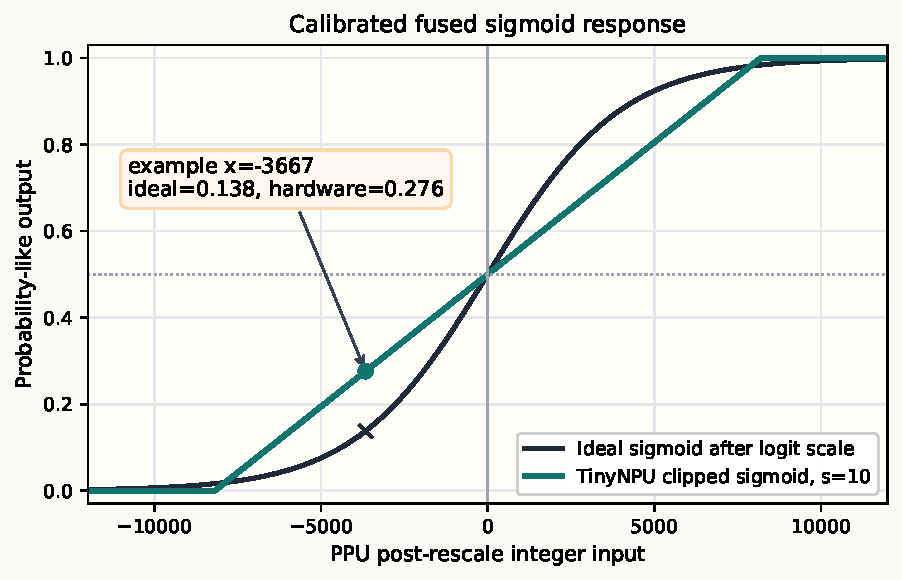
\includegraphics[width=0.96\linewidth]{figures/iszero_sigmoid_calibrated_comparison.pdf}
    \caption{TinyNPU hard-sigmoid response for the MNIST is-zero MLP final layer. The plot compares the calibrated hardware gate with the ideal sigmoid implied by the calibrated logit scale.}
    \label{fig:iszero-hardware-sigmoid}
\end{figure}

\begin{algorithm}[H]
\caption{TinyNPU ReLU}
\begin{algorithmic}[1]
\Require Signed integer input $x_{in}$ after PPU rescale
\Ensure Signed integer ReLU result before final output-precision saturation
\State \Return $\max(x_{in}, 0)$
\end{algorithmic}
\end{algorithm}

\begin{figure}[H]
    \centering
    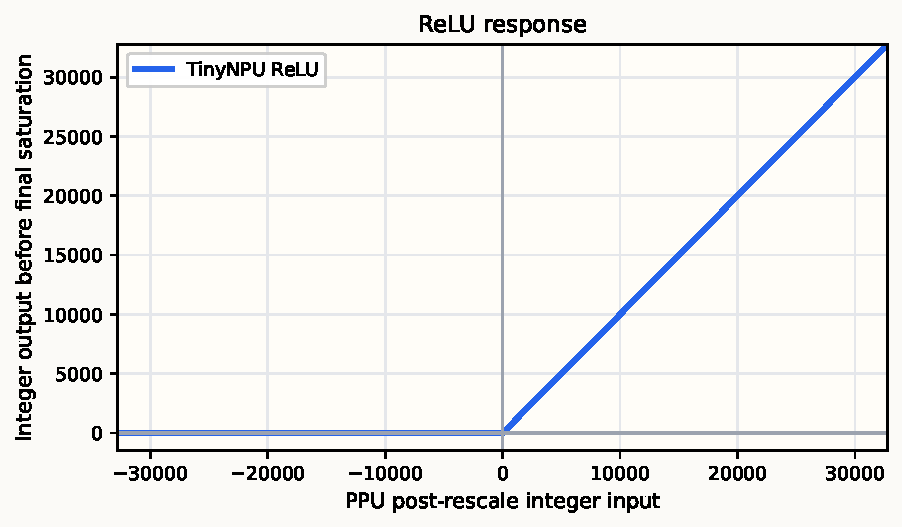
\includegraphics[width=0.82\linewidth]{figures/ppu_relu_response.pdf}
    \caption{TinyNPU ReLU response after PPU rescale and before final output-precision saturation.}
    \label{fig:ppu-relu-response}
\end{figure}

\begin{algorithm}[H]
\caption{TinyNPU Hard-GELU}
\begin{algorithmic}[1]
\Require Signed integer input $x_{in}$ after PPU rescale, activation-domain shift $k_x$
\Ensure Signed integer hard-GELU result in the same activation domain
\State $S \gets 2^{k_x}$
\State $g \gets ((218 \cdot x_{in} + 64) \gg 7) + 3S$
\State $g \gets \min(\max(g, 0), 6S)$
\State $u \gets (x_{in} \cdot g \cdot 10923 + 2^{15}) \gg 16$
\If{$k_x > 0$}
    \State $y \gets \textsc{RoundShiftSigned}(u, k_x)$
\Else
    \State $y \gets u$
\EndIf
\State \Return $y$
\end{algorithmic}
\end{algorithm}

The hard-GELU form is the place where the MobileNetV3 analogy is most direct. Standard GELU can be approximated as \(x\cdot\sigma(1.702x)\). The TinyNPU PPU replaces that sigmoid gate with a clipped affine gate, giving the integer-domain equivalent of
\[
    y \approx x \cdot \frac{\mathrm{clip}(1.703x + 3, 0, 6)}{6}.
\]
This matches the deployment idea behind MobileNetV3 hard-swish, but with the slope chosen to approximate GELU's sigmoid gate rather than swish's \(\sigma(x)\) gate.

\begin{figure}[H]
    \centering
    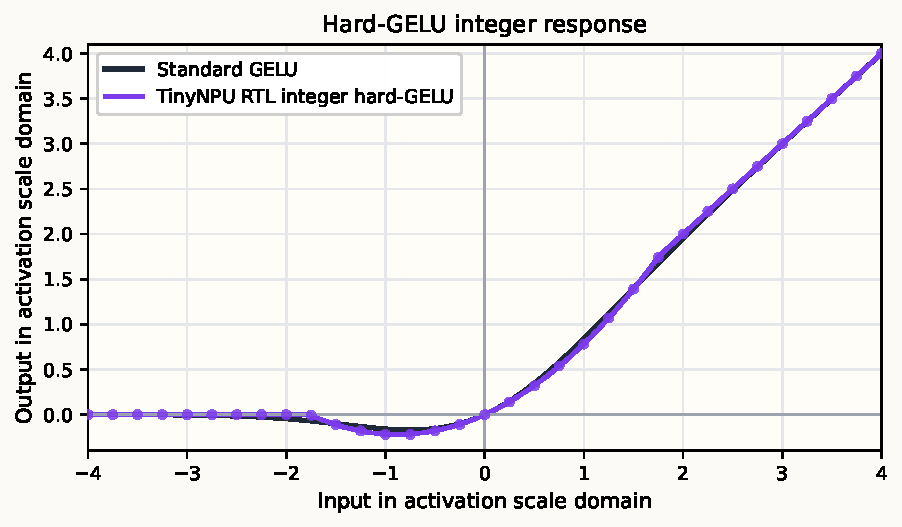
\includegraphics[width=0.82\linewidth]{figures/ppu_h_gelu_response.pdf}
    \caption{TinyNPU hard-GELU response in the activation scale domain. The purple curve is the RTL integer approximation from the staged PPU datapath; the black curve is standard floating-point GELU, included only as a shape reference.}
    \label{fig:ppu-h-gelu-response}
\end{figure}

\newpage
\bibliographystyle{plain}
\bibliography{references} 

\end{document}
